%%%%% --------------------------------------------------------------------------------
%%
%%                               Document Template
%%
%%%%% --------------------------------------------------------------------------------
%% Copyright (C) Huangrui Mo <huangrui.mo@gmail.com> 
%% This is free software: you can redistribute it and/or modify it
%% under the terms of the GNU General Public License as published by
%% the Free Software Foundation, either version 3 of the License, or
%% (at your option) any later version.
%%%%% --------------------------------------------------------------------------------
%%
%%%%************************ Document Class Declaration ******************************
%%
\documentclass[doublesided]{Style/ucasthesis}% thesis template of UCAS
%% Multiple optional arguments:
%% [scheme = plain] % for thesis writing of international students
%% [<singlesided|doublesided|printcopy>] % single-sided, double-sided, or print layout
%% [draftversion] % show draft version information, default is no show
%% [fontset = <adobe|...>] % specify font set, default is automatic detection
%% [standard options for ctex class]
%%%%% --------------------------------------------------------------------------------
%%
%%%%************************* Command Define and Settings ****************************
%%
\usepackage[myhdr]{Style/commons}% common settings
%% usage: \usepackage[option1,option2,...,optionN]{commons}
%% Multiple optional arguments:
%% [<numbered|authoryear|alpha>] % citation and reference style
%% <numbered>: textual: Jones [1]; parenthetical: [1]. default style
%% <authoryear>: textual: Jones (1995); parenthetical: (Jones, 1995)
%% <alpha>: textual: not available; parenthetical: [Jon95]
%% [myhdr] % one available header and footer style, will enable fancyhdr
%% [lscape] % provide landscape layout environment
%% [geometry] % configure page layout by geometry package
%% [list] % enable enhanced list environments, useful for Algorithm and Coding
%% [color] % enable color package to use color, default package is xcolor
%% [background] % enable page background, will auto enable color package
%% [tikz] % enable tikz for complex diagrams, will auto enbale color package
%% [table] % enable a table package for complex tables, default is ctable
%% [math] % enable some extra math packages
\usepackage{Style/custom}% user defined commands
%%%%% --------------------------------------------------------------------------------
%%
%%%%******************************** Content *****************************************
%%
\begin{document}
%%
%%%%% --------------------------------------------------------------------------------
%%
%%%%******************************** Frontmatter *************************************
%%
%% Frontmatter of Title page, Table of contents, Preface chapter.
\frontmatter
%%
%% >>> Frontpages
%%
%%
%%% >>> Title Page
%%
%%
%%% Chinese Title Page
%%
  \confidential{}% show confidential tag
  \schoollogo{scale=0.112}{UCAS}% university logo
  \title[社交网络中内容流行度预测研究]{社交网络中内容流行度预测研究}% \title[short title for headers]{Long title of thesis}
  \author{高金华}% name of author
  \advisor{李国杰~院士}% names and titles of supervisors
  \advisorinstitute{中国科学院计算技术研究所}% institute names of supervisors
  \degree{博士}% degree
  \degreetype{工学}% degree type
  \major{计算机系统结构}% major
  \institute{中国科学院计算技术研究所}% institute of author
  %\chinesedate{2014~年~06~月}% only need for user customized date
%%
%%% English Title Page
%%
  \englishtitle{Popularity Prediction for Online Content in Social Networks}
  \englishauthor{Gao Jinhua}
  \englishadvisor{Academician Li Guojie}
  \englishdegree{Doctor of Philosophy}
  \englishthesistype{Dissertation}
  \englishmajor{Computer Architecture}
  \englishinstitute{Institute of Computing Technology,\\Chinese Academy of Sciences}
  %\englishdate{June, 2014}% only need for user customized date
%%
%%% Generate Chinese Title
%%
\maketitle
%%
%%% Generate English Title
%%
\makeenglishtitle
%%
%%% >>> Author's declaration
%%
\makedeclaration
%%
%%% >>> Abstract
%%
\chapter{摘\quad 要}% does not show the title on the top
%\begin{abstract}% will show the title on the top
本文是中国科学院大学学位论文模板ucasthesis的使用说明文档。主要内容为介绍\LaTeX{}文档类ucasthesis的用法,以及如何使用\LaTeX{}快速高效地撰写学位论文。

\keywords{中国科学院大学,学位论文,\LaTeX{}模板}
%\end{abstract}


\chapter{Abstract}% does not show the title on the top
%\begin{englishabstract}% will show the title on the top
This paper is a help documentation for the \LaTeX{} class ucasthesis, which is  a thesis template for the University of Chinese Academy of Sciences. The main content is about how to use the ucasthesis, as well as how to write thesis efficiently by using \LaTeX{}.

\englishkeywords{University of Chinese Academy of Sciences (UCAS), Thesis, \LaTeX{} Template}
%\end{englishabstract}

%%
%%% >>> List of Content
%%
\intotoc{\contentsname}% add a corresponding item to the contents table and bookmark
\tableofcontents% contents catalog
\intotoc{\listfigurename}% add a corresponding item to the contents table and bookmark
\listoffigures% figures catalog
\intotoc{\listtablename}% add a corresponding item to the contents table and bookmark
\listoftables% tables catalog
%%
%% >>> prematter
%%
%%
%% >>> Nomenclatures
%%
\chapter{符号列表}

\section*{Characters}
\nomenclatureitem[\textbf{Unit}]{\textbf{Symbol}}{\textbf{Description}}
\nomenclatureitem[$\Unit{m^{2} \cdot s^{-2} \cdot K^{-1}}$]{$R$}{the gas constant}
\nomenclatureitem[$\Unit{m^{2} \cdot s^{-2} \cdot K^{-1}}$]{$C_v$}{specific heat capacity at constant volume}
\nomenclatureitem[$\Unit{m^{2} \cdot s^{-2} \cdot K^{-1}}$]{$C_p$}{specific heat capacity at constant pressure}
\nomenclatureitem[$\Unit{m^{2} \cdot s^{-2}}$]{$E$}{specific total energy}
\nomenclatureitem[$\Unit{m^{2} \cdot s^{-2}}$]{$e$}{specific internal energy}
\nomenclatureitem[$\Unit{m^{2} \cdot s^{-2}}$]{$h_T$}{specific total enthalpy}
\nomenclatureitem[$\Unit{m^{2} \cdot s^{-2}}$]{$h$}{specific enthalpy}
\nomenclatureitem[$\Unit{kg \cdot m \cdot s^{-3} \cdot K^{-1}}$]{$k$}{thermal conductivity}
\nomenclatureitem[$\Unit{K}$]{$T$}{temperature}
\nomenclatureitem[$\Unit{s}$]{$t$}{time}
\nomenclatureitem[$\Unit{kg \cdot m^{-1} \cdot s^{-2}}$]{$p$}{thermodynamic pressure}
\nomenclatureitem[$\Unit{kg \cdot m^{-1} \cdot s^{-2}}$]{$\hat{p}$}{hydrostatic pressure}
\nomenclatureitem[$\Unit{kg \cdot m^{-2} \cdot s^{-2}}$]{$\Vector{f}_b$}{body force}
\nomenclatureitem[$\Unit{m^2}$]{$\mathrm{S}$}{boundary surface}
\nomenclatureitem[$\Unit{m^3}$]{$\mathrm{V}$}{volume}
\nomenclatureitem[$\Unit{m \cdot s^{-1}}$]{$\Vector{V}$}{velocity vector}
\nomenclatureitem[$\Unit{m \cdot s^{-1}}$]{$u$}{x component of velocity}
\nomenclatureitem[$\Unit{m \cdot s^{-1}}$]{$v$}{y component of velocity}
\nomenclatureitem[$\Unit{m \cdot s^{-1}}$]{$w$}{z component of velocity}
\nomenclatureitem[$\Unit{m \cdot s^{-1}}$]{$c$}{speed of sound}
\nomenclatureitem[$\Unit{m}$]{$\Vector{r}$}{position vector}
\nomenclatureitem[$\Unit{1}$]{$\unitVector{n}$}{unit normal vector}
\nomenclatureitem[$\Unit{1}$]{$\hat{\unitVector{t}}$}{unit tangent vector}
\nomenclatureitem[$\Unit{1}$]{$\tilde{\unitVector{t}}$}{unit bitangent vector}
\nomenclatureitem[$\Unit{1}$]{$C_R$}{coefficient of restitution}
\nomenclatureitem[$\Unit{1}$]{$Re$}{Reynolds number}
\nomenclatureitem[$\Unit{1}$]{$Pr$}{Prandtl number}
\nomenclatureitem[$\Unit{1}$]{$Ma$}{Mach number}
\nomenclatureitem[$\Unit{m^2 \cdot s^{-1}}$]{$\alpha$}{thermal diffusivity}
\nomenclatureitem[$\Unit{kg \cdot m^{-1} \cdot s^{-1}}$]{$\mu$}{dynamic viscosity}
\nomenclatureitem[$\Unit{m^2 \cdot s^{-1}}$]{$\nu$}{kinematic viscosity}
\nomenclatureitem[$\Unit{1}$]{$\gamma$}{heat capacity ratio}
\nomenclatureitem[$\Unit{kg \cdot m^{-3}}$]{$\rho$}{density}
\nomenclatureitem[$\Unit{kg \cdot m^{-1} \cdot s^{-2}}$]{$\sigma_{ij}$}{stress tensor}
\nomenclatureitem[$\Unit{kg \cdot m^{-1} \cdot s^{-2}}$]{$S_{ij}$}{deviatoric stress tensor}
\nomenclatureitem[$\Unit{kg \cdot m^{-1} \cdot s^{-2}}$]{$\tau_{ij}$}{viscous stress tensor}
\nomenclatureitem[$\Unit{1}$]{$\delta_{ij}$}{Kronecker tensor}
\nomenclatureitem[$\Unit{1}$]{$I_{ij}$}{identity tensor}

\section*{Operators}
\nomenclatureitem{\textbf{Symbol}}{\textbf{Description}}
\nomenclatureitem{$\Delta$}{difference}
\nomenclatureitem{$\nabla$}{gradient operator}
\nomenclatureitem{$\delta^{\pm}$}{upwind-biased interpolation scheme}

\section*{Abbreviations}
\nomenclatureitem{\textbf{Acronym}}{\textbf{Description}}
\nomenclatureitem{ANFO}{Ammonium Nitrate Fuel Oil}
\nomenclatureitem{CFD}{Computational Fluid Dynamics}
\nomenclatureitem{CFL}{Courant-Friedrichs-Lewy}
\nomenclatureitem{CJ}{Chapman-Jouguet}
\nomenclatureitem{EOS}{Equation of State}
\nomenclatureitem{JWL}{Jones-Wilkins-Lee}
\nomenclatureitem{TVD}{Total Variation Diminishing}
\nomenclatureitem{WENO}{Weighted Essentially Non-oscillatory}
\nomenclatureitem{ZND}{Zel'dovich-von Neumann-Doering}

% list of symbols, preface of books
%%
%%%%% --------------------------------------------------------------------------------
%%
%%%%******************************** Mainmatter **************************************
%%
%% Main topics.
\mainmatter
%%
%%% >>> Main Contents
%%
%%%%% --------------------------------------------------------------------------------
%%
%%%%******************************* Main Content *************************************
%%
%%% ++++++++++++++++++++++++++++++++++++++++++++++++++++++++++++++++++++++++++++++++++
\chapter{引言}
\label{chap:introduction}

\section{研究背景与意义}
\section{研究现状}
\section{面临的挑战}
\section{本文的工作}
\subsection{研究目标和内容}
\subsection{研究成果}
\subsection{论文的组织结构}


\chapter{相关研究综述}
\label{chap:relatedwork}
流行度预测问题自被提出以来,受到了学术界和产业界的广泛关注。本章从流行度的统计特征分析、流行度预测方法以及流行度预测问题的可预测性三个方面入手,对流行度预测领域的相关工作进行了系统的总结和归纳,以便读者更好地了解和掌握该领域的相关知识,进而更好地理解本文的工作。

\section{流行度的统计特征分析}
在线内容的流行度分析工作最早源于网站缓存策略的研究。Cunha等人\citep{cunha1995characteristics}在研究站点中网页的访问情况时发现,网页被访问频率的分布服从Zipf定律\citep{zipf2016human},也就是说:流行度排名为$i$的网页被用户访问的概率正比于$1/i$,如图\ref{fig:pageDist}所示。这一现象表明,网页的访问频次分布是不均匀的。Almeida等人\citep{almeida1996characterizing}在研究万维网中所有网页的访问频次时,也发现了同样的分布规律。
\begin{figure}[!htbp]
  \centering
  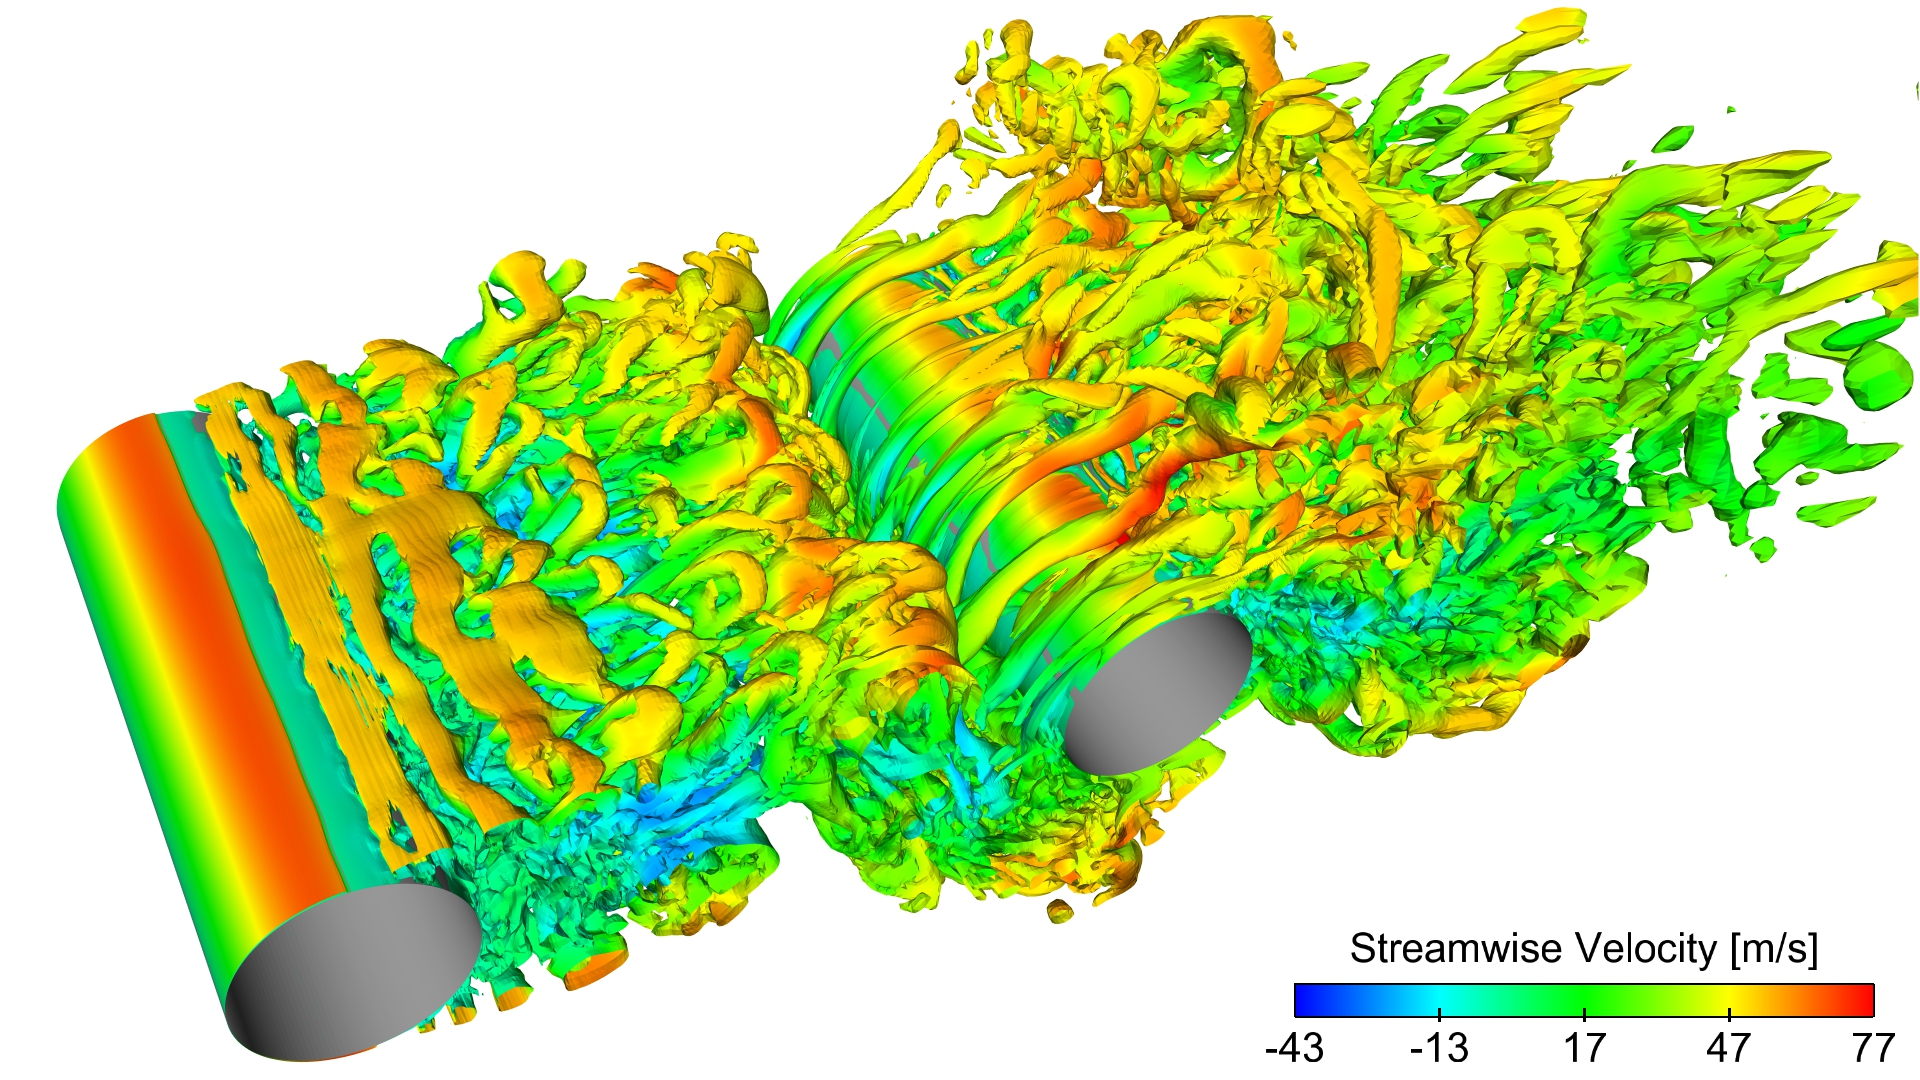
\includegraphics[width=0.45\textwidth]{ITC_Q_Criteria}
  \caption{Q判据等值面图}
  \label{fig:pageDist}
\end{figure}

随着信息技术的发展,视频分享类网站和社交网络平台不断涌现,也引起了研究人员的关注。Gill等人\citep{gill2007youtube}收集并分析了视频网站Youtube\footnote{\url{https://www.youtube.com}}上视频的访问数据,发现视频的访问频次信息依然服从Zipf定律。Cha等人\citep{cha2009analyzing}对Youtube网站上的视频数据进行了详细的分析,发现网站中不同类别下的视频的观看数分布都服从幂律分布。Kwak等人\citep{kwak2010twitter}研究了社交网络平台Twitter\footnote{\url{https://twitter.com}}上消息的转发情况,发现参与消息转发的人数服从幂律分布,如图\ref{fig:tweetDist}所示。
\begin{figure}[!htbp]
  \centering
  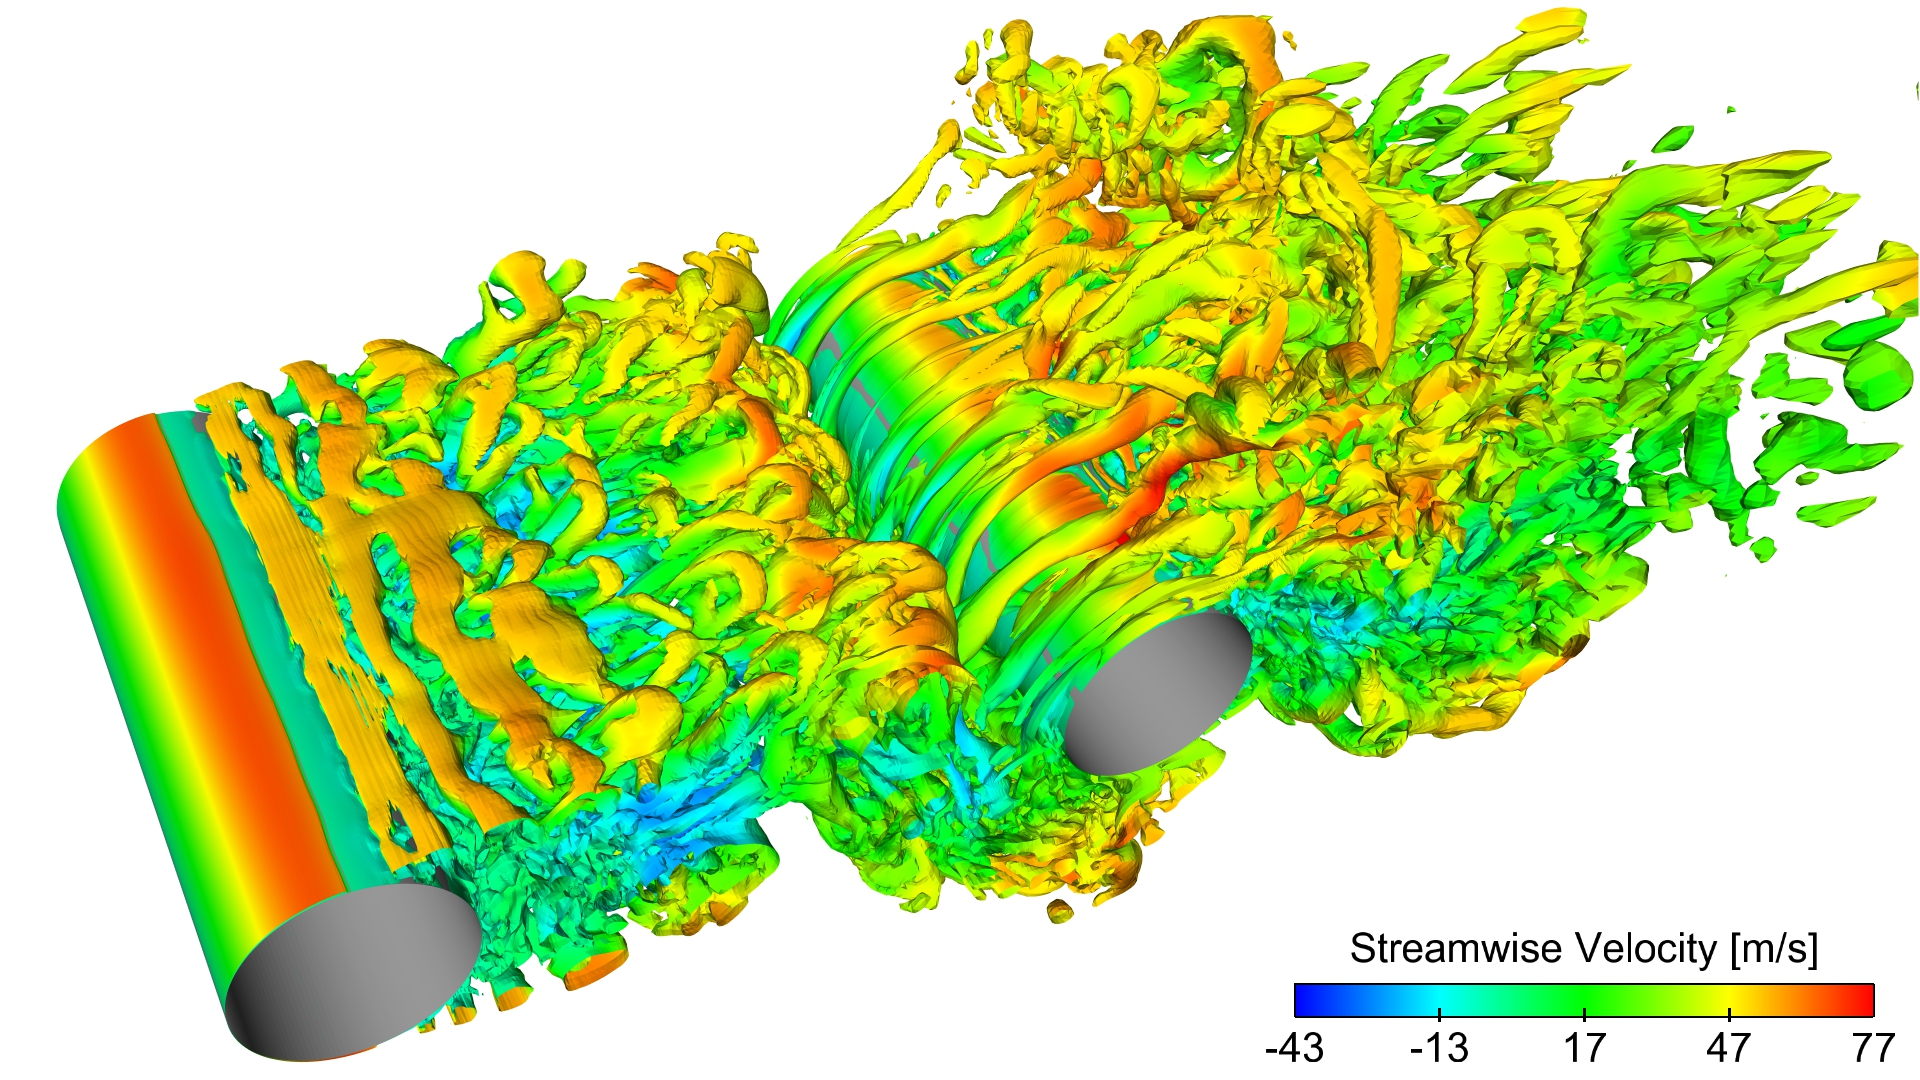
\includegraphics[width=0.45\textwidth]{ITC_Q_Criteria}
  \caption{Q判据等值面图}
  \label{fig:tweetDist}
\end{figure}

除了对宏观的流行度统计量的分析之外,还有一部分工作研究了流行度增长过程中的微观统计特征。Barabasi等人\citep{barabasi05}研究了人类的行为数据,发现人类的行为模式并不是服从传统方法中假设的泊松过程,而是存在爆发现象,并提出了一种基于事件优先级的排队模型来解释这一现象。爆发现象是指人类在参与某类事件时,大部分时间都处于沉寂状态,不会采取任何行为动作;中间夹杂了少数爆发区域,在爆发区域内会有大量的行为数据产生,如图\ref{fig:burst}所示。

爆发现象在在线内容的流行度增长过程中十分常见。Kaltenbrunner等人\citep{kaltenbrunner2007description}研究了新闻评论网站Slashdot\footnote{\url{https://slashdot.org}}上新闻的评论情况,并对评论数据的时间间隔分布进行了分析。统计结果表明,评论数据的时间间隔分布是两个log-normal分布的混合,并且存在明显的周期现象。Bao等人\citep{bao2013cumulative}研究了新浪微博中消息的转发时间间隔数据,发现转发时间间隔分布服从幂律分布,这也说明了社交网络中消息的流行度累积过程中存在爆发现象。
\begin{figure}[!htbp]
  \centering
  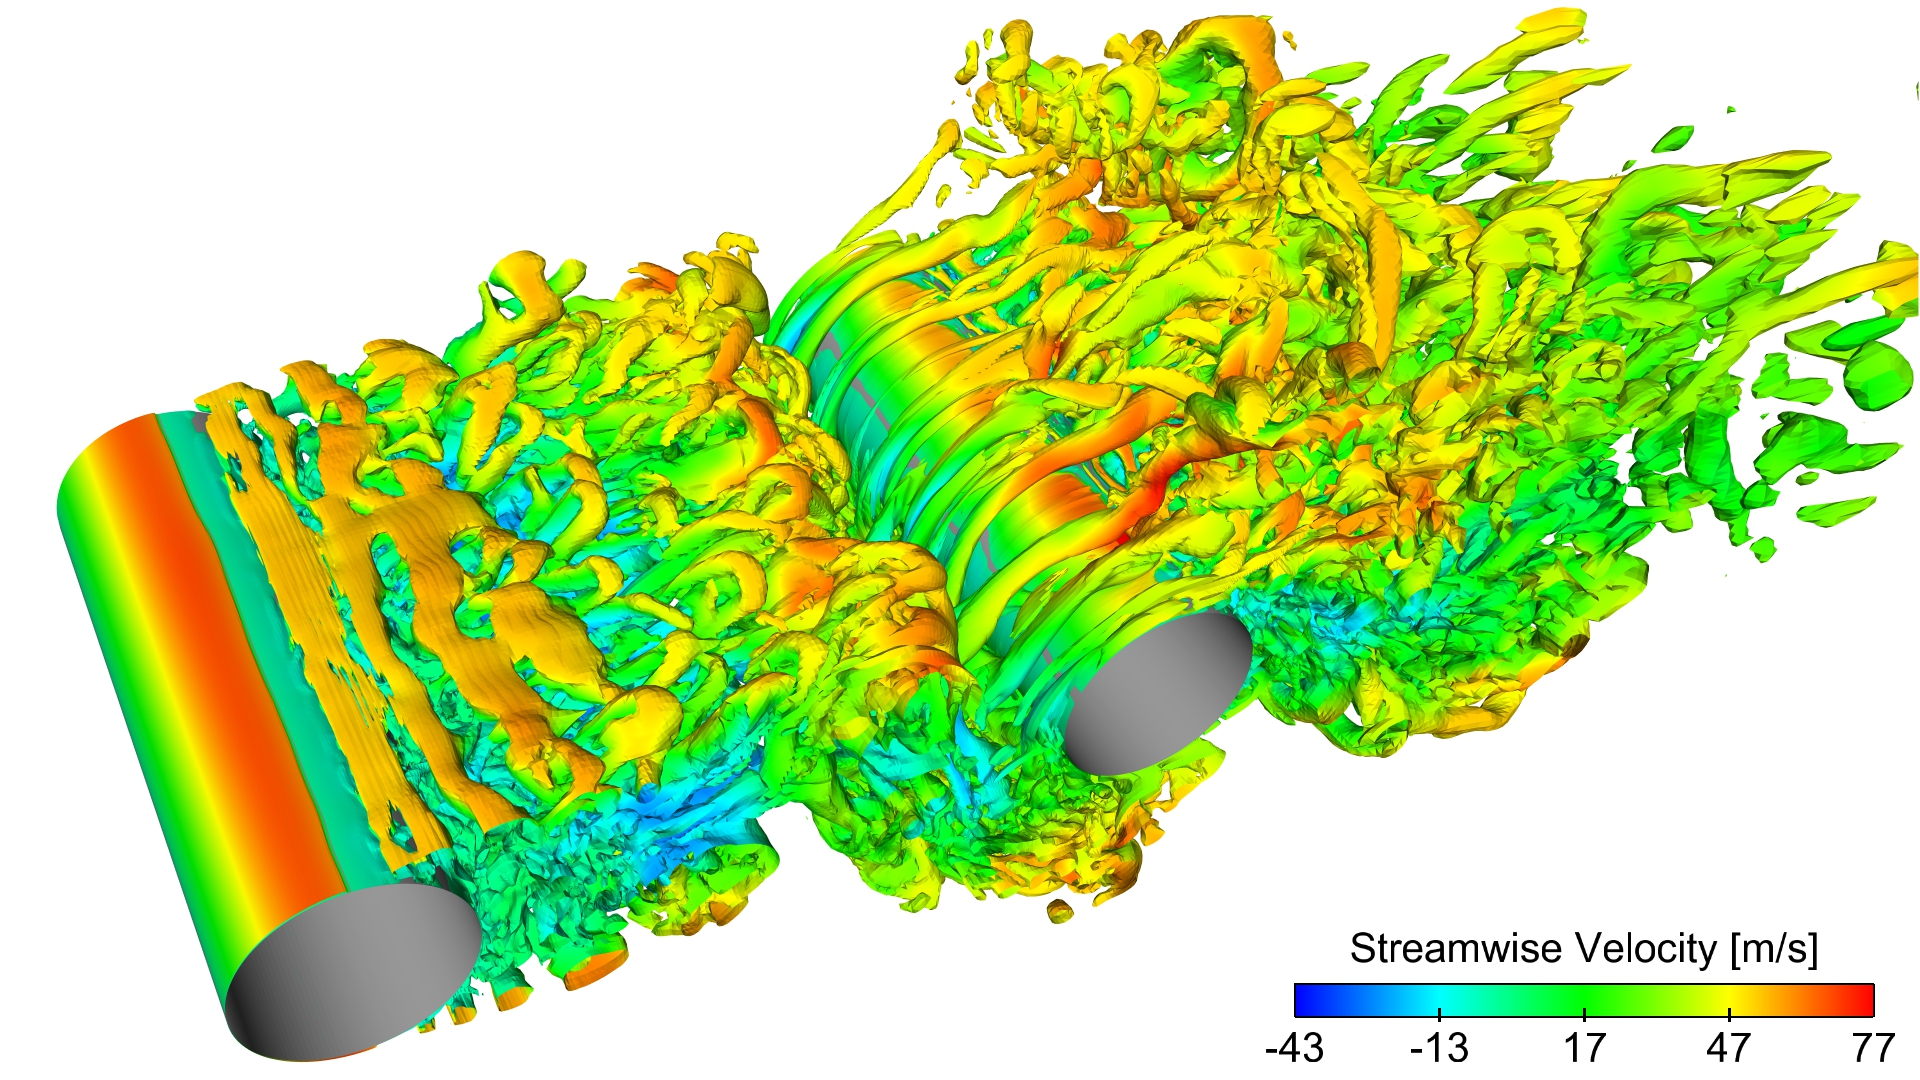
\includegraphics[width=0.45\textwidth]{ITC_Q_Criteria}
  \caption{Q判据等值面图}
  \label{fig:burst}
\end{figure}

除爆发现象外,研究人员还发现流行度的增长过程中存在着固定的模式。Yang等人\citep{yang2011patterns}研究了Twitter平台上消息的传播过程,提出了K-SC(K-Spectral Centroid)聚类方法,对消息的流行度变化过程进行聚类,将消息的流行度变化过程聚为六类,如图\ref{fig:pattern}所示。Crane等人\citep{crane2008robust}在研究Yotube网站中视频的观看数据时发现,视频的观看到达时间服从幂律分布,呈现出明显的``爆发-衰落"现象。此外,Costa等人\citep{ferraz2015rsc}还发现流行度的增长过程中呈现出明显的周期性特点。
\begin{figure}[!htbp]
  \centering
  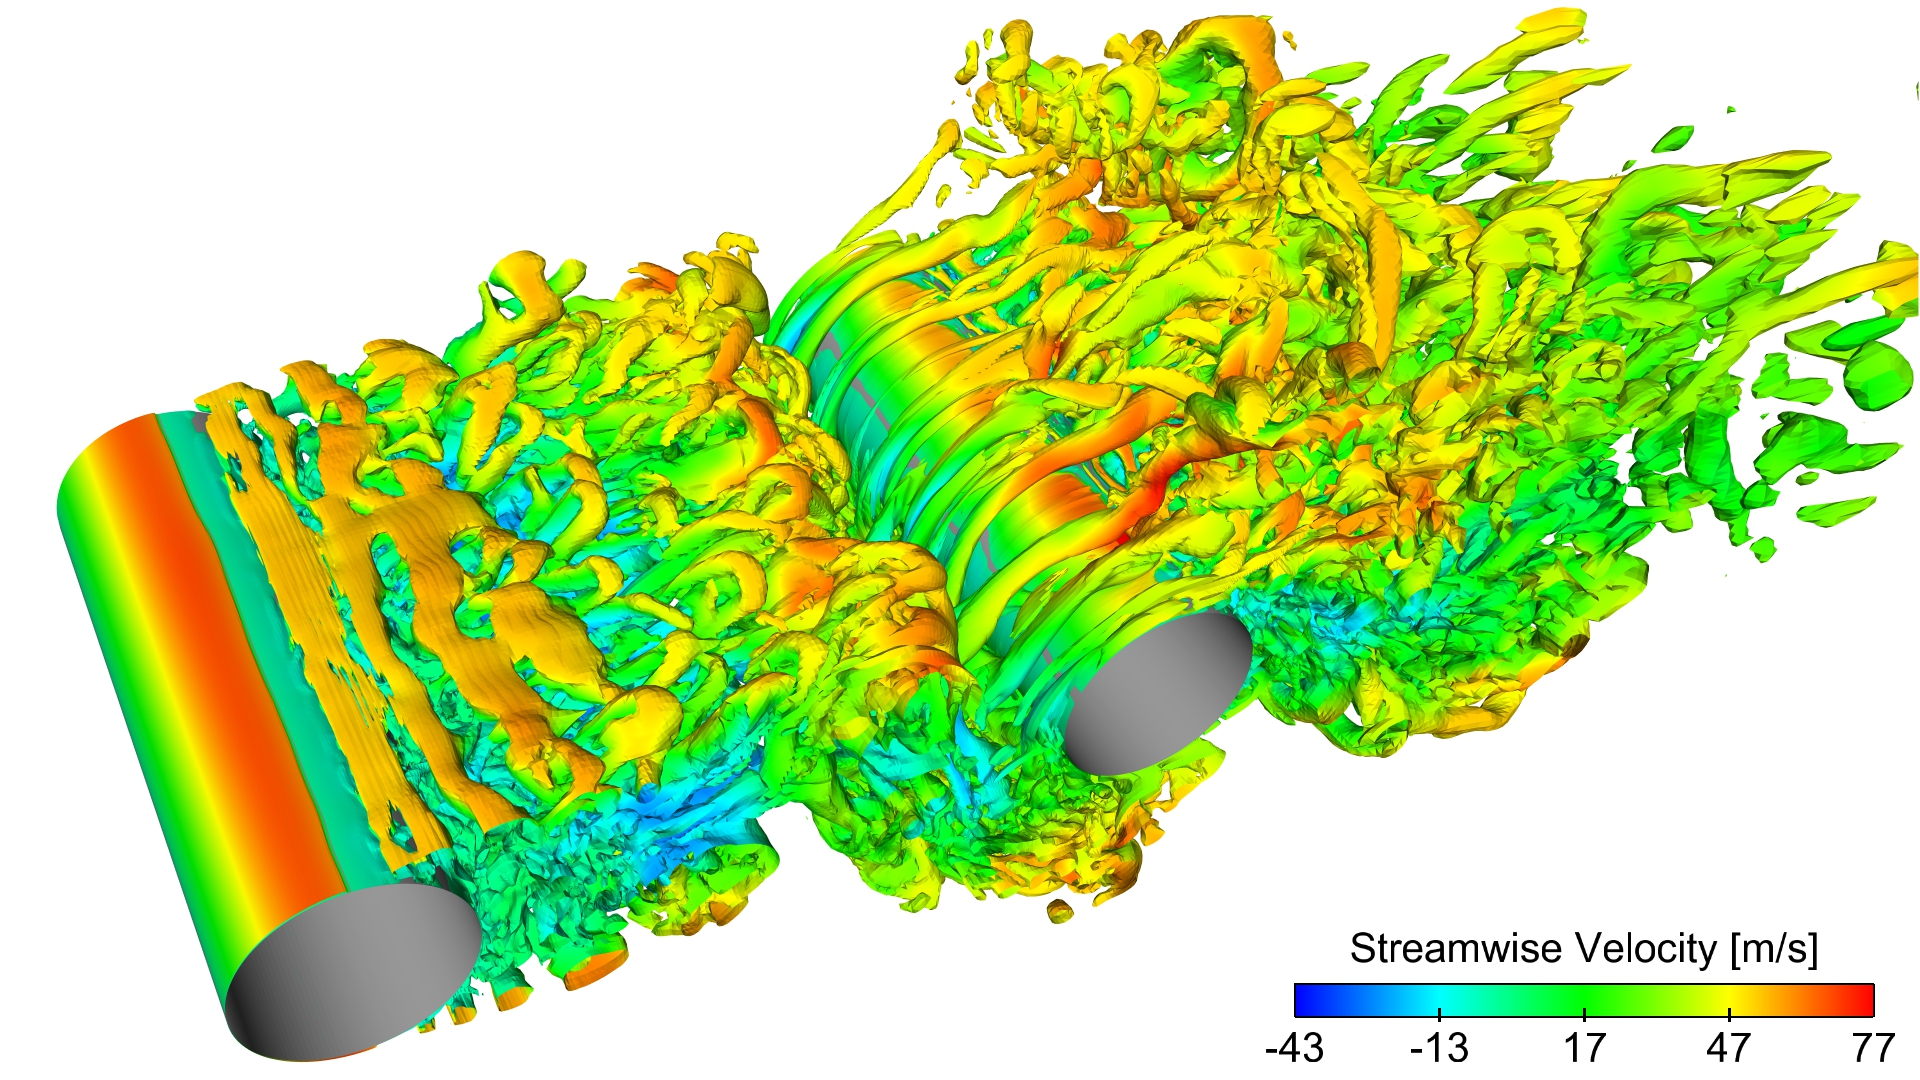
\includegraphics[width=0.45\textwidth]{ITC_Q_Criteria}
  \caption{Q判据等值面图}
  \label{fig:pattern}
\end{figure}

流行度分布的不均匀性,以及增长过程出现的爆发现象和时序特性,吸引了大量研究人员的关注,进而涌现出了多种流行度预测的模型和方法。
\section{流行度预测方法概述}
现有的流行度预测方法主要包含三类:基于特征的有监督学习方法、基于点过程的流行度到达过程建模方法和基于表示学习的方法。本节会依次对这三类方法进行介绍和总结。
\subsection{基于特征的有监督学习方法}
基于特征的流行度预测方法主要通过借助已有的有监督学习模型,结合人工抽取的特征,来对流行度的增长过程进行预测。在这类方法中,流行度预测问题通常会被形式化为分类或者回归问题:给定一组历史消息的各种特征信息以及消息在观测窗口$[0,T_r]$和预测窗口$[0,T_s]$内的流行度数据作为训练样本,利用现有的分类或回归方法学习得到预测模型,进而对待预测的消息的流行度作出预测。这类方法的核心在于寻找对于流行度预测有着重要指示作用的特征。常见的用于流行度预测的特征包括消息内容特征、用户特征、时序特征和传播级联的结构特征。
\begin{figure}[!htbp]
  \centering
  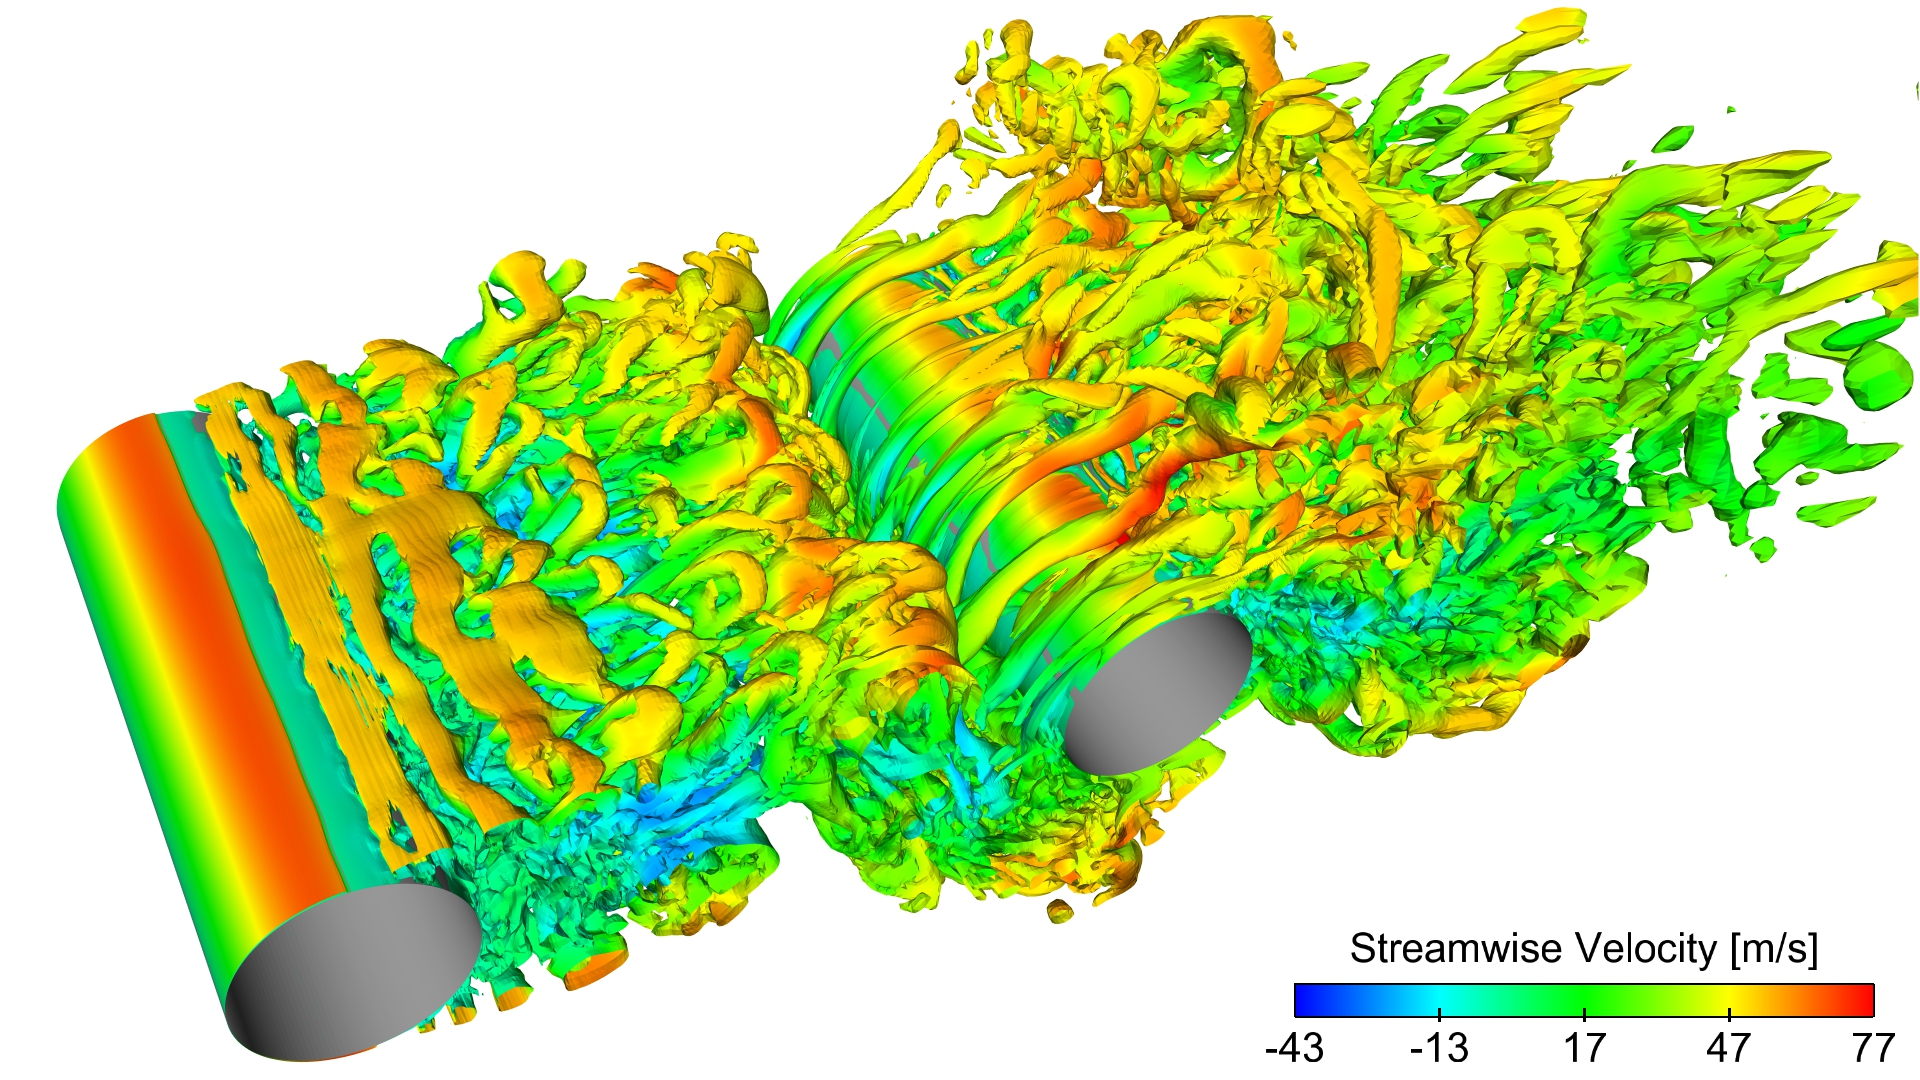
\includegraphics[width=0.45\textwidth]{ITC_Q_Criteria}
  \caption{Q判据等值面图}
  \label{fig:loglinear}
\end{figure}

时序特征方面,常用于流行度预测的时序特征包括观测窗口内的累积流行度特征和流行度时间序列特征。Cha等人\citep{cha2009analyzing}分析了Youtube网站上视频的流行度增长数据,发现视频上传7天后的访问量和视频上传后一天以及上传后两天的访问量之间存在着非常强的相关性,进而提出了预测视频近期流行度的任务,并指出视频上传后短期内的累计流行度是重要的指示特征。Szabo等人\citep{szabo2010predicting}研究了Digg\footnote{\url{http://digg.com}}网站上的新闻数据和Youtube网站上的视频数据,发现这些内容早期的流行度和后期的流行度在进行对数变换后,存在着非常强的线性相关性,如图\ref{fig:loglinear}所示。基于这一观测,作者提出了S-H(Szabo-Huberman)模型,将消息在观测窗口内的累积流行度作为特征,利用对数线性回归模型来预测消息在预测时刻的流行度。Gursun等人\citep{gursun2011describing}分析了Youtube网站中部分视频在上传后一年内完整的观看频次序列,发现可以根据将视频按照访问频次分为两类:长期流行的视频和短期流行的视频,并利用时间序列分析模型中的自回归移动平均模型(Autoregressive Moving Average,ARMA)\citep{marple1987digital},对长期流行的视频的流行度变化过程进行了预测。Pinto等人\citep{pinto2013using}研究了Youtube网站中视频的流行度时间序列数据。作者将视频在观测窗口等分为若干长度相等的区间,并抽取了各时间区间内视频的观看数的增长量作为特征。作者在研究视频的时间序列后发现S-H模型的假设存在着局限性:早期累计流行度相近的视频,后期的流行度变化过程可能会有很大的差距,如图\ref{fig:pinto}所示。作者提出将消息在观测窗口内的时间序列数据作为特征,利用多元线性回归模型来预测消息的流行度。
\begin{figure}[!htbp]
  \centering
  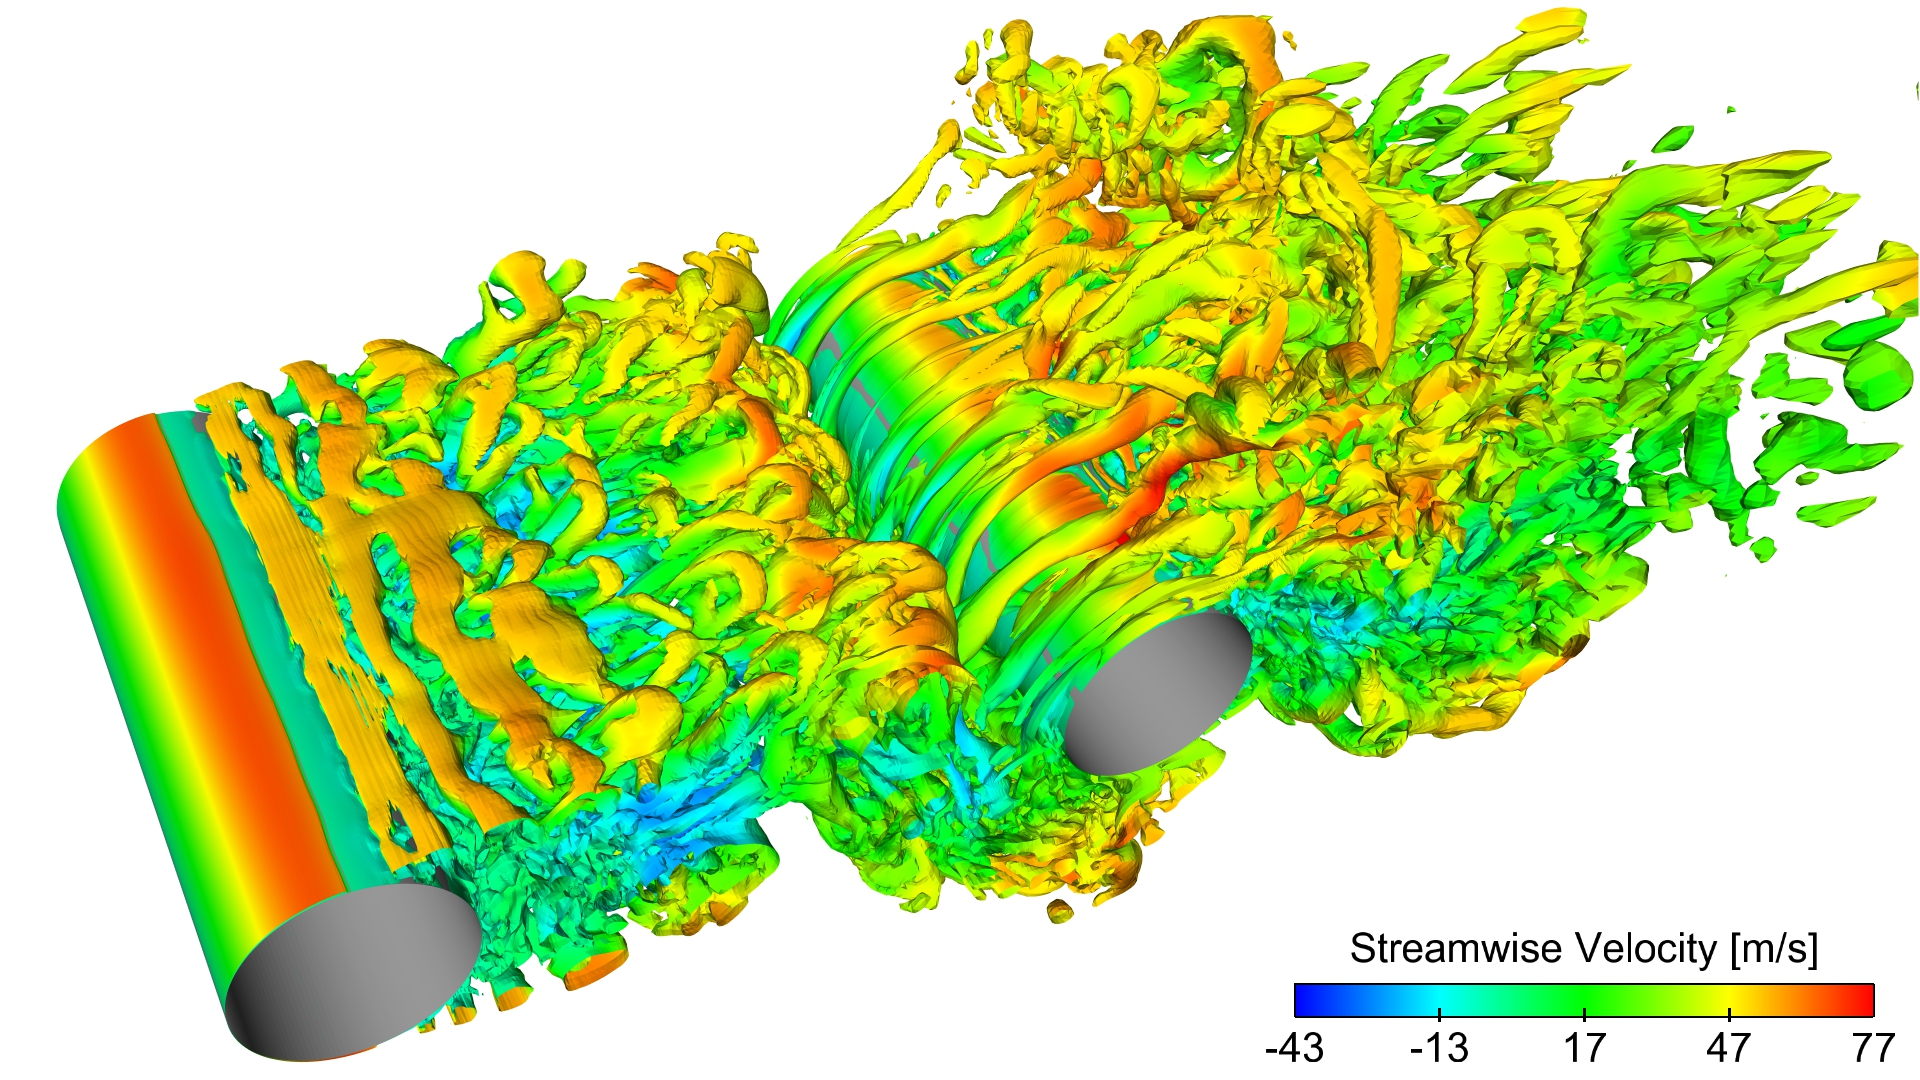
\includegraphics[width=0.45\textwidth]{ITC_Q_Criteria}
  \caption{Q判据等值面图}
  \label{fig:pinto}
\end{figure}

内容特征方面,Tsagkias等人\citep{tsagkias2009predicting}抽取了新闻的内容特征,来对新闻的评论数进行事前预测:在新闻发布之前,利用新闻的元信息,来预测新闻的评论数。作者将这一预测问题形式化为两阶段分类问题:新闻发布能否接收到评论,以及接收到的评论数会高还是低。在特征方面,作者抽取了新闻中重要性较高的前100个词的词频信息作为新闻的文本特征,新闻中包含的不同类型的命名实体的个数作为新闻的语义特征。此外,作者还抽取了新闻的其他元信息特征。实验结果表明,文本特征和语义特征对分类结果有较好的指示作用。Hong等人\citep{hong2011predicting}同样将Twitter平台中消息的流行度预测问题形式化为一个两阶段分类问题:消息是否会被转发以及消息最终的流行度等级。作者利用TF-IDF模型和LDA主题模型\citep{blei2003latent}来抽取消息的内容特征,同时结合网络拓扑结构特征以及时序特征来进行预测。Bandari等人\citep{bandari2012pulse}研究了新闻订阅站点Feedzilla\footnote{\url{http://news.feedzilla.com}}的数据在Twitter平台上的流行度情况。作者抽取了新闻的四类内容特征来进行预测,包括新闻所属的类别、新闻源站点的信息、新闻的倾向性特征和新闻中包含的命名实体。作者分别使用回归和分类模型对新闻的流行度进行了预测,得到了很好的预测效果。Bian等人\citep{bian2014predicting}研究了腾讯微博\footnote{\url{http://t.qq.com}}中消息的传播情况和用户的参与情况,从兴趣导向、社交影响和病毒式传播三个方面,建模了用户和消息之间的相互作用,进而对消息的流行度和用户的参与情况进行预测。建模过程中,作者提出了一种多任务迁移模型来建模消息的内容,提取出消息中的主题信息,用于后续的预测任务。

用户特征方面,最常见的用户特征是用户在社交网络中的拓扑结构信息,例如Twitter平台中用户的粉丝数和关注数信息\citep{gupta2012predicting,zhao2013short,kupavskii2013predicting,kong2014predicting}。用户的某些元信息也会被提取作为特征,包括用户账号的创建时长、用户历史发布的消息数\citep{suh2010want}、视频网站中的用户类别\citep{borghol2012untold}等。Yang等人\citep{yang2010modeling}在研究Twitter平台上消息的传播情况时,考虑了用户间的相互影响,提出了一种线性影响力模型。该模型可以在网络拓扑结构未知的情况下,来刻画用户间的影响力。Cui等人\citep{cui2013cascading}在研究Twitter平台上的消息爆发预测时,直接将用户身份作为特征。消息爆发预测问题旨在于给定消息在观测窗口内的流行度变化情况,预测消息最终的流行度能否达到爆发的阈值。作者在建模时借助于传感器的思想,将网络中所有的用户都当作传感器,只需要根据部分关键传感器的激活状态,即用户是否参与消息转发,就可以来判断消息最终能否爆发。因此,作者将爆发预测问题形式化为一个二分类问题,以所有的用户为特征,将用户在观测窗口内的激活状态转化成0-1向量作为输入,以消息最终的爆发情况作为输出,训练得到一个二分类器,进而对待预测的消息进行预测。

传播级联的结构特征方面,Bao等人\citep{bao2013popularity}分析了新浪微博中消息的传播级联情况,重点研究了传播级联形成的转发树的深度和链接密度情况,发现这两个特征与流行度的变化之间存在着非常强的相关性。作者将这两个因素加入到S-H模型中,发现预测精度得到了很大的提升。

除上述四类特征之外,研究人员还探寻了很多其他因素对流行度的影响。Brodersen等人\citep{brodersen2012youtube}研究了Youtube视频的观看数与地理因素之间的关系。Jenders等人\citep{jenders2013analyzing}研究了内容的情感倾向性对Twitter平台中消息转发数的影响。Weng等人\citep{weng2013virality}研究了流行度与网络的社区结构之间的关系,Junus等人\citep{junus2015community}也将社区结构因素建模到流行度预测模型中。此外,还有工作考虑了用户有限的关注度对流行度的影响\citep{hodas2012visibility,weng2012competition}。

问题形式化方面,不同于传统工作中将流行度预测形式化为一个回归或者分类问题,Cheng等人\citep{cheng2014can}将流行度预测问题形式化为阶段性的增长预测问题。作者指出,在以往的流行度分类预测问题中,由于流行度本身的分布是幂律的,导致各个类别样本数极度不均匀,从而影响最终的预测效果。因此,作者提出了``$kto2k$"问题:给定当前流行度为$k$的消息,预测它们最终的流行度能否增长到$2k$。基于样本集中流行度的分布,作者证明了提出的``$kto2k$"问题是一个均衡的二分类问题,并抽取了内容特征、用户特征、网络结构特征以及时序特征来进行预测。实验结果表明,随着$k$的增长,分类预测的准确率也在不断提高。

综上所述,基于特征的有监督学习方法在进行流行度预测时,关键在于抽取出会影响流行度变化的特征,但是特征工程是一项非常耗时耗力的工作,而且很大程度上受限于研究人员的先验认识。

\subsection{基于点过程的流行度到达过程建模方法}
基于点过程的流行度到达过程建模方法主要是在生存分析理论\citep{klein2005survival}的框架下进行的。这类方法中常见的流行度预测问题定义如下:给定一条消息$m$在观测窗口$[0,T]$内每一次转发的时间戳序列$C^m=\{t_i^m|0=t_0^m \le t_1^m \le...\le t_N^m \le T \}$作为输入,其中$N$表示消息$m$在观测窗口内总的转发次数,$t_i^m$表示消息$m$的第$i$次转发的转发时间与消息$m$的源发时间的间隔;最终的目标是预测后续流行度随时间的变化情况。这类方法通常将流行度的增长过程形式化为一个计数过程(Counting process)\citep{andersen1985counting}:使用随机过程$\{N(t),t \ge 0\}$来刻画消息累积流行度随时间$t$变化的序列,其中$N(t)$取值是非负整数,且满足单调性:$N(s) \le N(t), \forall s \le t$。在生存分析理论框架下来建模$N(t)$序列时,关键在于对强度函数(Intensity function)的刻画。强度函数$x(t)$刻画了在给定历史信息$H_t=\{t_i|t_i < t \}$时,时间区间$[t,t+dt]$内有新事件发生的概率,即:
\begin{equation}
\label{eq:intensity}
P\{event \enspace happens \enspace in \enspace [t,t+dt] \enspace | \enspace H_t\}=x(t)dt\text{,}
\end{equation}
$\mathbb{E}_{dN(t)\~{0,1}}[dN(t)|H_t]=x(t)dt$,从而将计数序列$N(t)$与强度函数$x(t)$之间的关系用如下微分方程来刻画:
\begin{equation}
\label{eq:differential}
\frac{\mathbb{E}[dN(t)]}{dt}=x(t)\text{。}
\end{equation}


\subsection{基于表示学习的方法}
\subsection{其他方法}
\section{流行度预测问题的可预测性分析}


\chapter{基于相似微博的流行度预测方法}
\label{chap:three}
\section{引言}
流行度预测在站点优化、广告策划以及市场营销等领域有着重要的应用意义。现有的流行度预测方法主要可以归结为三类:基于特征的有监督学习方法、基于随机过程的方法和基于表示学习的方法。基于特征的方法主要是通过人工提取大量与流行度变化相关的特征,以历史消息的传播数据为样本,学习得到流行度预测函数;基于随机过程的方法则是在生存分析理论的框架下,设计流行度增长过程的强度函数,从而对流行度的到达过程进行建模;基于表示学习的方法则是受深度学习领域的影响,利用深度模型来建模影响流行度变化的因素。这三类方法的详细介绍可参加本论文的第二章。

现有的三类方法在对流行度进行预测时,存在一个共同的缺陷:对历史消息没有进行充分地挖掘和利用。人们对社交网络平台的深度使用,也使得我们积累了大量的历史传播数据。这些历史传播数据中蕴含了丰富的信息,包括消息的不同传播模式信息以及流行度的增长变化信息等,但是现有的方法没有对这部分数据进行充分地利用。基于随机过程的方法通常只是以待预测消息在观测窗口内的转发数据作为输入,而没有显示地利用历史消息;基于有监督学习的方法则是将所有的历史消息作为训练样本,学习得到一个平均的模型。这样的模型没有充分考虑历史数据中不同消息间的差异性以及离群点的影响。因此,本章研究内容的出发点就是设计一种能够充分利用历史数据的流行度预测模型。

近邻思想是机器学习领域的一种重要思想。它的基本出发点是利用样本间的相似性来对样本进行处理,在分类问题和回归问题中都有着重要的应用,例如常用分类问题中常用的$k$--NN模型\citep{keller1985fuzzy}和回归问题中的高斯随机过程方法\citep{williams1996gaussian}都是基于近邻的思想。流行度预测问题同样可以从近邻的角度去考虑。海量的历史传播数据为我们提供了大量的样本。对于待预测的消息,我们可以从海量的历史样本中寻找出与之相近的历史样本,并利用历史样本的流行度变化信息,来对待预测消息的流行度变化进行预测。

 在本章中,我们提出了一种基于相似消息的流行度预测方法。对于待预测的消息,我们根据它在观测窗口内的流行度增长过程,从历史消息中寻找出与之相似的部分消息,再基于相似消息来对该消息后续的流行度变化进行预测。在定义消息之间的相似度时,我们将消息传播中包含的传播模式作为隐变量,利用文本领域的主题模型\citep{blei2003latent}学习得到消息在不同传播模式上的分布来作为消息的表达,进而使用余弦距离来度量消息之间的相似度。我们的方法既充分利用了历史信息,同时也考虑了消息本身传播过程的特异性。在数据集上的实验结果表明,我们的方法在流行度预测任务上要明显优于前两类方法。

\section{相关工作}
流行度预测研究领域的工作非常多,前面提到的基于特征的有监督学习方法、基于随机过程的方法和基于表示学习的方法在第二章中已有详细介绍,这里不再赘述。本节主要介绍一些基于消息间的相似性开展的流行度预测工作。

Kong等人\citep{kong2014predicting}提出了kSAIT模型对为微博平台中消息的转发数进行预测。作者假设同一用户发布的消息在传播过程上是相似的,并在此基础上提出了一种用户特定的转发数预测方法:针对每一个用户,学习得到一个独立的转发数预测函数。作者将用户历史发布的每一条消息在观测窗口内的传播数据中提取出一系列的特征来作为消息的表示。对于用户新发布的消息,作者先计算该消息与用户发布的历史消息之间的相似度,再根据相似度挑选出最高的$k$条历史消息,并根据选取的历史消息来对新发布消息的流行度进行预测。这种方法的先验假设过于理想,并且需要对每一个用户来学习不同的预测函数。此外,在对消息的表示上,需要人工提取特征,并不能真正体现消息在传播过程上的相似性。

基于消息分组思想的流行度预测方法也是对消息间相似度的一种隐式利用。Cao等人\citep{cao2017predicting}在微博数据集上对S--H模型\citep{szabo2010predicting}的适应性进了分析。作者先将所有的训练样本上训练,得到模型的参数;再根据消息在观测窗口的累积流行度,将训练样本分成不同的组别,然后在每个组别上分别训练得到S--H模型的参数。对比两组实验结果,作者发现,不同组别上学习得到的模型参数差异非常大,而且都与全部样本上训练得到的模型间存在着显著的差异。论文中的实验结果表明,`` 将所有的样本作为一个集合进行训练,再将训练得到的模型应用到所有的测试样本上"这样的预测框架在流行度预测问题上存在着明显的缺陷。因此,我们需要对训练样本进行更进一步的挖掘。Hoang等人\citep{hoang2017gpop}则是从用户分组的角度来考虑流行度预测问题。在完成用户分组后,作者也是利用了近邻的思想来对消息进行预测。作者从训练数据中选出与待预测消息相似的$k$条消息,再将这$k+1$条消息的传播数据组成一个三维张量,利用张量填充的方式来对待预测消息的流行度进行估计。
%已有的流行度预测方法大体可以分为两类:基于特征的方法和基于点过程的方法。
%
%基于特征的方法通常将流行度预测问题形式化为回归或分类问题,人工地定义和抽取大量特征,使用有监督的框架来学习特征到流行度之间的变换函数。Szabo等人[11]研究了Digg上的新闻数据和Youtube上的视频数据,发现这些内容早期的流行度和后期流行度之间存在着很强的对数线性相关,并将消息的早期累积流行度为特征,提出了SH(Szabo-Huberman)模型来预测消息的流行度。Pinto等人[12]在SH模型的基础上,将观测窗口内的累积流行度拆分为等长时间间隔内的流行度增长序列,利用多元回归模型来预测流行度。这类工作中,也有研究者专注于分析和发现对流行度预测有指示作用的特征。Suh等人[13]研究了Twitter平台上消息的转发情况,并抽取了一系列的特征来预测消息的最终转发数。实验结果表明,消息中包含的URL和hashtag标签信息,对消息转发数的预测有很重要的指示作用。消息发布者的元信息,包括粉丝数和关注数等,也与最终的预测结果存在很强的关联关系。Bao等人[14]研究了新浪微博上消息转发形成的转发树数据,提取了消息转发树的深度和连接密度两个特征,有效提高了回归模型的预测精度。此外,Cheng等人[15]将流行度预测问题形式化为阶段性的增长预测问题。他们指出,在以往的流行度分类预测问题中,由于流行度本身的分布是幂律的,导致各个类别样本数极度不均匀,从而影响最终的预测效果。因此,他们提出了“kto2k”问题:给定当前流行度为k的消息,预测它们最终的流行度能否增长到2k。 基于样本集中流行度的分布,他们证明了提出的“kto2k”问题是一个均衡的二分类问题,并抽取了内容特征、用户特征、网络结构特征以及时序特征来进行预测。实验结果表明,随着k的增长,分类预测的准确率也在不断提高。
%
%基于点过程的方法通常只利用待预测消息自身的信息,通过对待预测消息在观测窗口内流行度到达过程的建模,来预测消息后续流行度的变化。这类方法将流行度的增长过程形式化为一个计数过程[16](Counting process),并将强度函数(Intensity function)的刻画作为模型的核心。强度函数 刻画了给定历史信息 下,在时间窗口 内有新事件发生的概率,即:
% 。
%基于这一框架,Shen等人[3]提出了基于自增强泊松过程(Reinforced Poisson process, RPP)的RPP模型。在建模消息的强度函数时,考虑了消息本身的吸引力、时间衰减机制和富者愈富机制。Gao等人[4]将RPP模型应用到新浪微博中,并对几种机制的作用形式进行了修正。Bao等人[5]采用了自激励Hawkes过程(Self-exciting Hawkes process)来建模强度函数,刻画了消息传播过程中转发用户带来的激励作用。Zhao等人[17]在自激励过程的基础上,进一步引入了用户的影响力信息。他们将用户的粉丝数加入到强度函数的建模中,进一步提升了模型的预测效果。这类方法由于没有利用其他历史消息的信息,预测能力比较有限。
%
%此外,Mishra等人[18]提出了将上述两类方法融合的方法。他们先利用自激励过程来建模消息在观测窗口内的流行度增长过程,再将学习得到的参数与人工抽取的其他过程合并,利用回归模型来预测消息的最终流行度。近年来,深度学习的方法在流行度预测领域也取得了不错的的进展。Li等人[19] 提出了端到端的DeepCas模型。他们在监督学习框架下,先利用深度学习模型将消息在观测窗口内的转发情况表示为向量,再利用神经网络模型学习消息的流行度增长与转发向量间的转换函数。Cao等人[20]在自激励过程的启发下,提出了DeepHawkes模型。他们利用深度学习模型,刻画了传播过程中的用户影响力、用户激励以及时间衰减效应等影响因子,在数据集上取得了很好的预测效果。

\section{模型}
\subsection{问题形式化}
消息$i$在给定时间窗口$[0,T]$内的传播数据可以用时间戳序列$C^i=\{t_k^i|t_k^i<T,k=1,2,...,n_i\}$表示,其中$n_i$表示消息$i$在时间窗口内的转发次数,$t_k^i$表示第$k$次转发距离消息源发时间的间隔。给定一组历史消息在完整窗口$[0,T]$的传播数据和一组待预测消息在观测窗口 $[0,T_0]$($T_0<T$)的传播数据,我们需要对待预测消息在时间窗口$[T_0,T]$内的流行度变化进行预测。

\subsection{整体预测框架}
不同于传统的基于特征的方法和基于点过程的方法,我们提出了一种基于相似消息的流行度预测方法。我们对所有消息在观测窗口的传播数据进行表示,对于待预测的每一条消息$j$ ,我们在历史消息中找到与之相似的$K$条消息,利用这$K$条消息在窗口$[T_0,T]$内的数据,来预测消息$j$在预测窗口$[T_0,T]$内的流行度。我们提出的方法,既充分利用了历史消息的传播数据,同时又避免了对所有的消息使用统一的预测模型,充分考虑了消息传播过程的特异性。在我们的模型中,如何对消息的传播数据进行表示,进而找到与之相似的历史消息,是至关重要的部分。

\subsection{消息传播数据的表示}
时间序列$(x_1,x_2,...,x_N)$通常被用来将消息的传播数据转化为定长的向量化表示,其中 $N$表示划分的等长时间区间的个数,$x_i$表示在第$i$个时间间隔内流行度的增长量。这种时间序列的表示方式能一定程度上反应消息的流行度变化趋势,但是这种表示方法的效果受时间区间粒度的影响,同一条消息在不同大小的时间区间下的表示差异较大。另外,它也不能刻画消息在传播模式上的区别。事实上,消息的传播过程中包含着不同的传播模式,如快速爆发的模式、均匀增长的模式、逐渐衰退的模式等。图\ref{fig:example}中展示了两条示例消息的传播过程。从图中可以看到,在时间序列表示下,以5个单位时间为一个时间区间,两条消息的表达都是$(25,21)$,但是两条消息的传播过程并不相同。第一条消息经历了平稳增长和衰落的过程,可以预见后续的流行度增长量会比较小;而第二条消息在经历了第1个时间间隔内的快速增长和衰落后,在第2个时间间隔内又迎来了平稳增长的过程,后续的流行度应该会持续增加。因此,基于时间序列的表示方法,会忽略消息传播过程所包含的不同传播模式,难以真正捕获传播过程相似的消息用于预测。
\begin{figure}[!htbp]
  \centering
  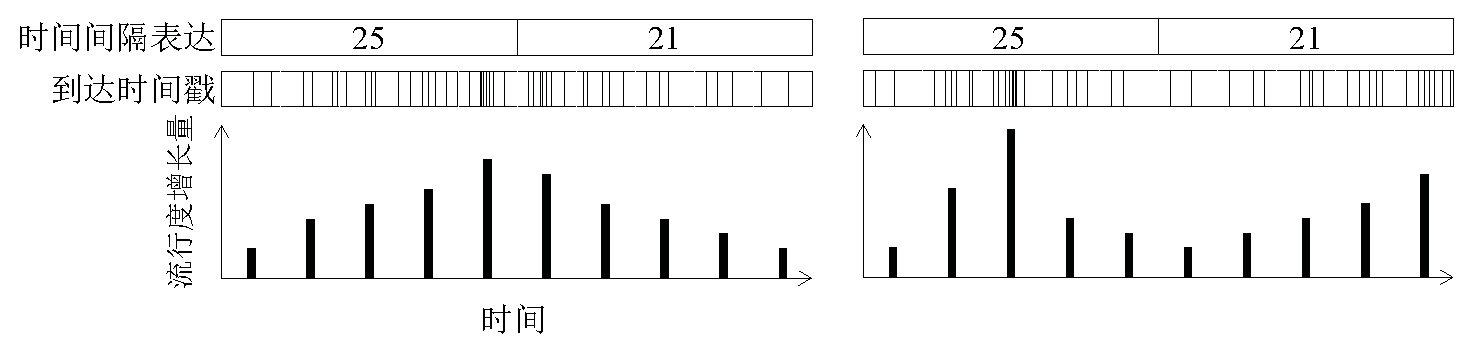
\includegraphics[width=1\textwidth]{3-example}
  \caption{两条示例消息的传播数据}
  \label{fig:example}
\end{figure}

进一步地观察图\ref{fig:example},我们可以发现:消息在处于不同的传播模式时,转发到达的速率不同,形成的转发时间间隔的分布也不相同。当消息处于快速爆发的模式时,会产生大量的短时间间隔;而当消息处于衰退模式时,会产生较少但是持续时间长的转发时间间隔。因此,消息在传播过程中产生的时间间隔数据,可以帮助推断消息所处的传播模式。
我们将消息的传播过程类比于文档的产生过程,利用文档主题模型来学习消息传播数据的表示。我们将消息的传播模式类比于文档的主题,消息转发过程中产生的时间间隔类比于文档中的词。每个消息的传播数据可以表示为在不同传播模式上的分布。我们统计了数据集中转发时间间隔的分布,结果如图\ref{fig:intervalDist}所示。从图中可以发现,转发时间间隔的分布与文档集中词的分布是类似的,都服从幂律分布。
\begin{figure}[!htbp]
  \centering
  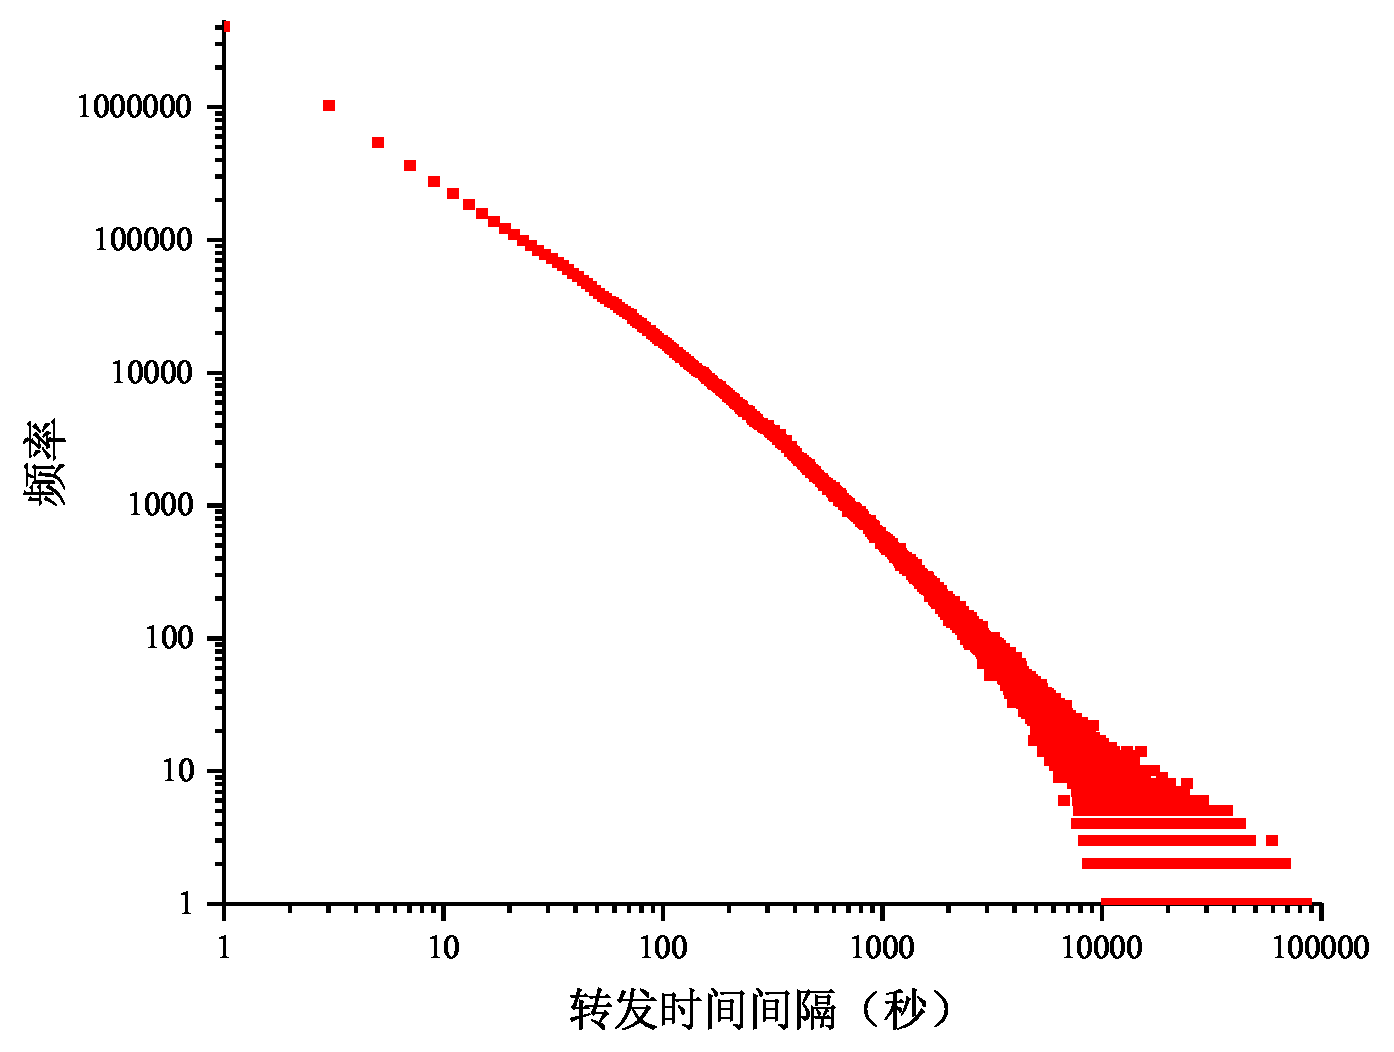
\includegraphics[width=0.8\textwidth]{3-IntervalDist}
  \caption{数据集中消息转发时间间隔的分布}
  \label{fig:intervalDist}
\end{figure}

对于一条消息$i$,它的第$k$个转发时间间隔$\Delta t_k^i$定义为$\Delta t_k^i=t_k^i-t_{k-1}^i$。 类似于LDA模型,我们采用如下的产生过程来生成$\Delta t_k^i$:
\begin{itemize}
\item	消息$i$根据自身传播模式的分布,采样一个传播模式$P$;
\item	根据传播模式$P$下产生时间间隔的分布,采样得到$\Delta t_k^i$。
\end{itemize}

我们采用了LDA模型来从时间间隔数据中学习得到消息传播模式的分布,将其作为消息的表示。在模型学习时,我们将消息在观测窗口$[0,T_0]$内的数据$C^i=\{t_k^i|t_k^i<T,k=1,2,...,n_i\}$转成时间间隔 $\{\Delta t_k^i|\Delta t_k^i=t_k^i-t_{k-1}^i,k=1,2,...,n_i\}$。每条消息的时间间隔数据作为一个文档,所有训练数据集中出现过的时间间隔的集合作为词汇表。另外,我们方法使用了绝对的时间间隔数据,避免了时间序列表示方法中时间区间粒度的问题。

\subsection{消息流行度预测}
在学习得到消息的表示之后,我们提出了一种基于相似消息的流行度预测方法。对于每一条待预测消息$j$,我们首先利用训练集上学习得到的LDA模型,推断它在不同传播模式下的分布作为它的表示,然后计算它与训练集中所有历史消息的相似程度,选取出相似度最高的$K$条历史消息。对于每个待预测的时间点,我们将抽取的$K$条历史消息在该时间点的流行度求取平均值,作为消息$j$在该时间点的流行度的预测。为了避免离群点对预测结果的影响,我们使用截尾均值[21](Trimmed mean)作为平均值的计算方式。截尾均值的定义为:在计算序列$\{s_1,s_2,...,s_N\}$的截尾均值时,先将该序列按照从小到大的顺序排列,得到$\{\widetilde{s_1},\widetilde{s_2},...,\widetilde{s_N}\}$;再去掉序列中最大的$\varepsilon$\%数据和最小的$\varepsilon$\%数据,将剩余数据的均值作为序列的截尾均值。其中$\varepsilon$是待设置的参数。

我们模型的整体预测框架如图\ref{fig:architecture} 所示。
\begin{figure}[!htbp]
  \centering
  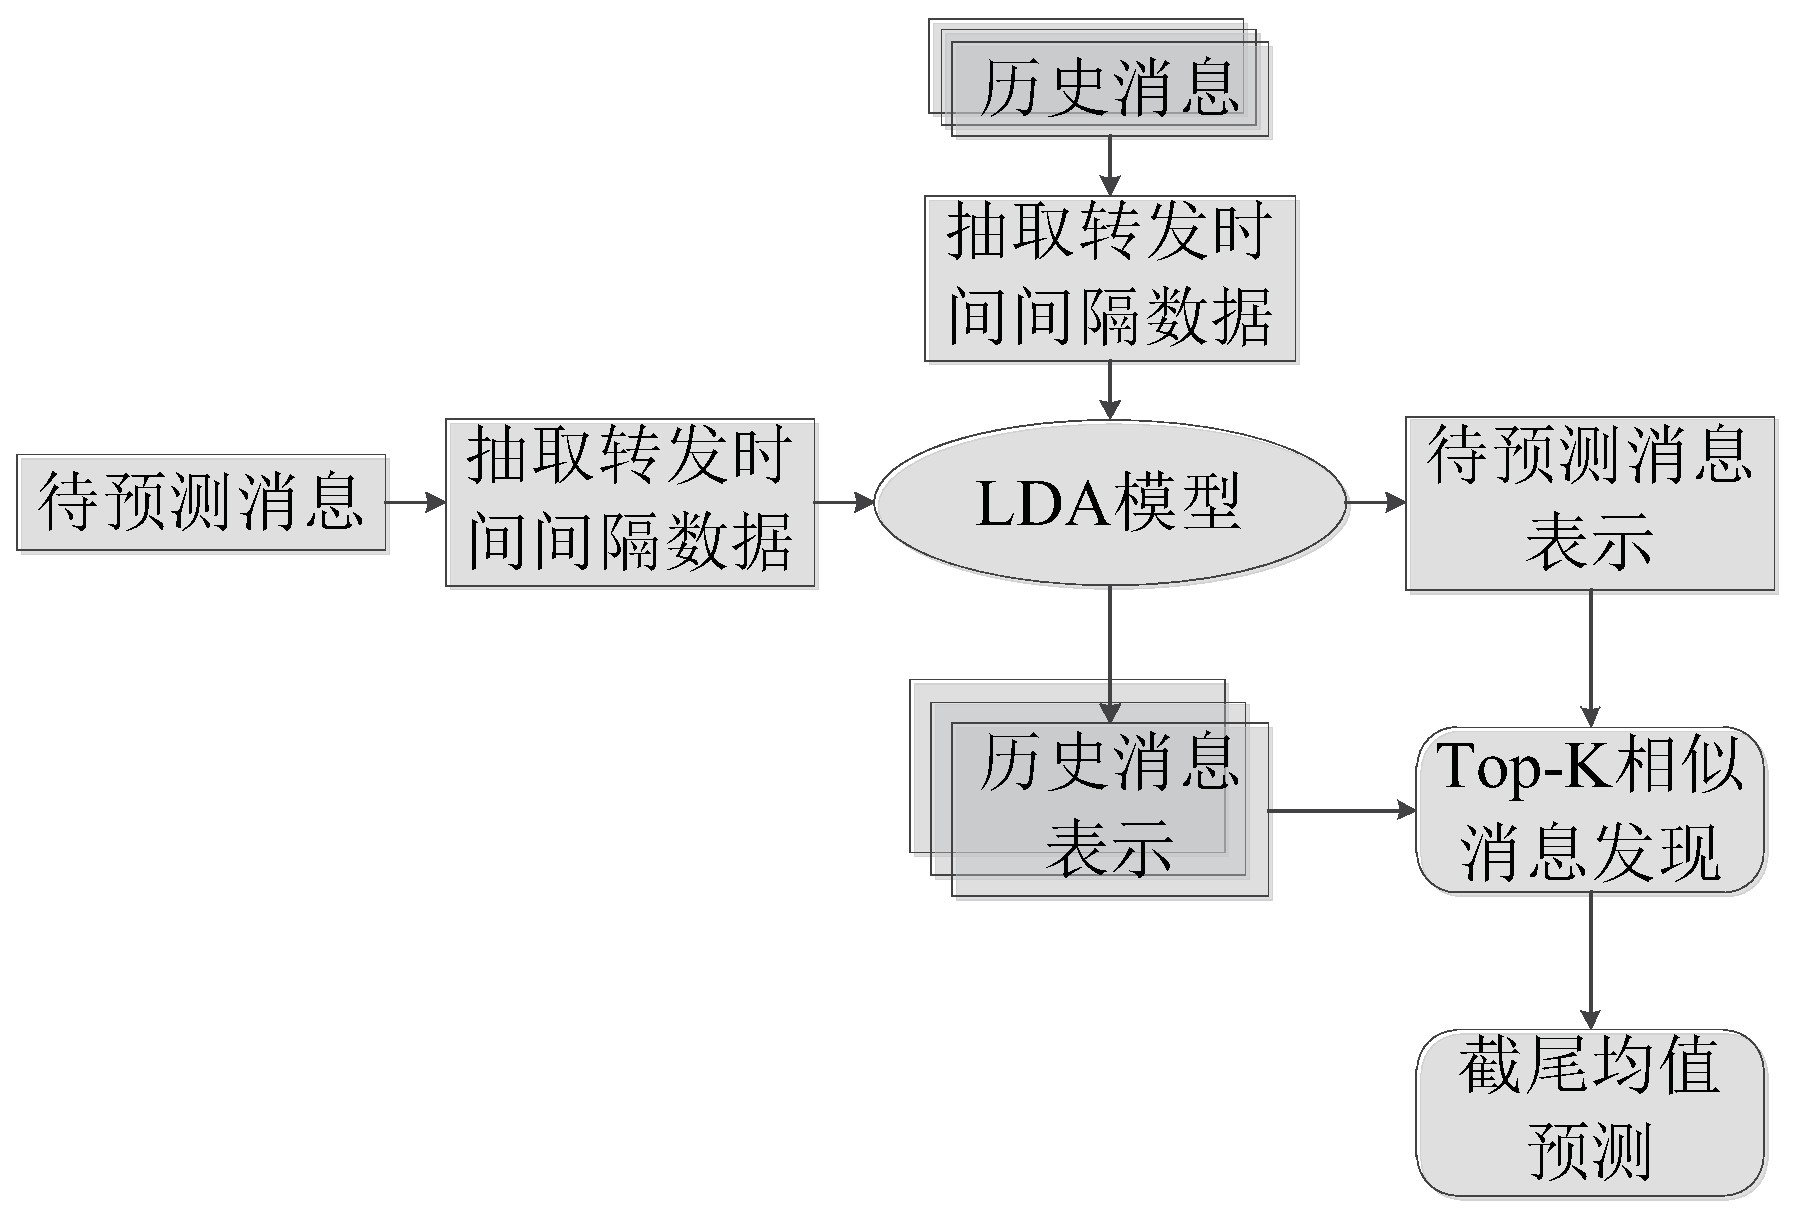
\includegraphics[width=0.8\textwidth]{3-architecture}
  \caption{模型的整体预测框架}
  \label{fig:architecture}
\end{figure}

\section{实验}
\subsection{实验数据}
我们抓取了微博上某一天的全部源发消息和它们发布后24小时内的转发数据来作为我们的实验数据。我们过滤了发布1小时后累计转发数小于10的消息,最终用于实验的数据集包含了6.5万条源发消息和它们在发布后24 小时内的转发数据。我们统计了数据集中微博的流行度分布,结果如图\ref{fig:retweetDist}所示。
\begin{figure}[!htbp]
  \centering
  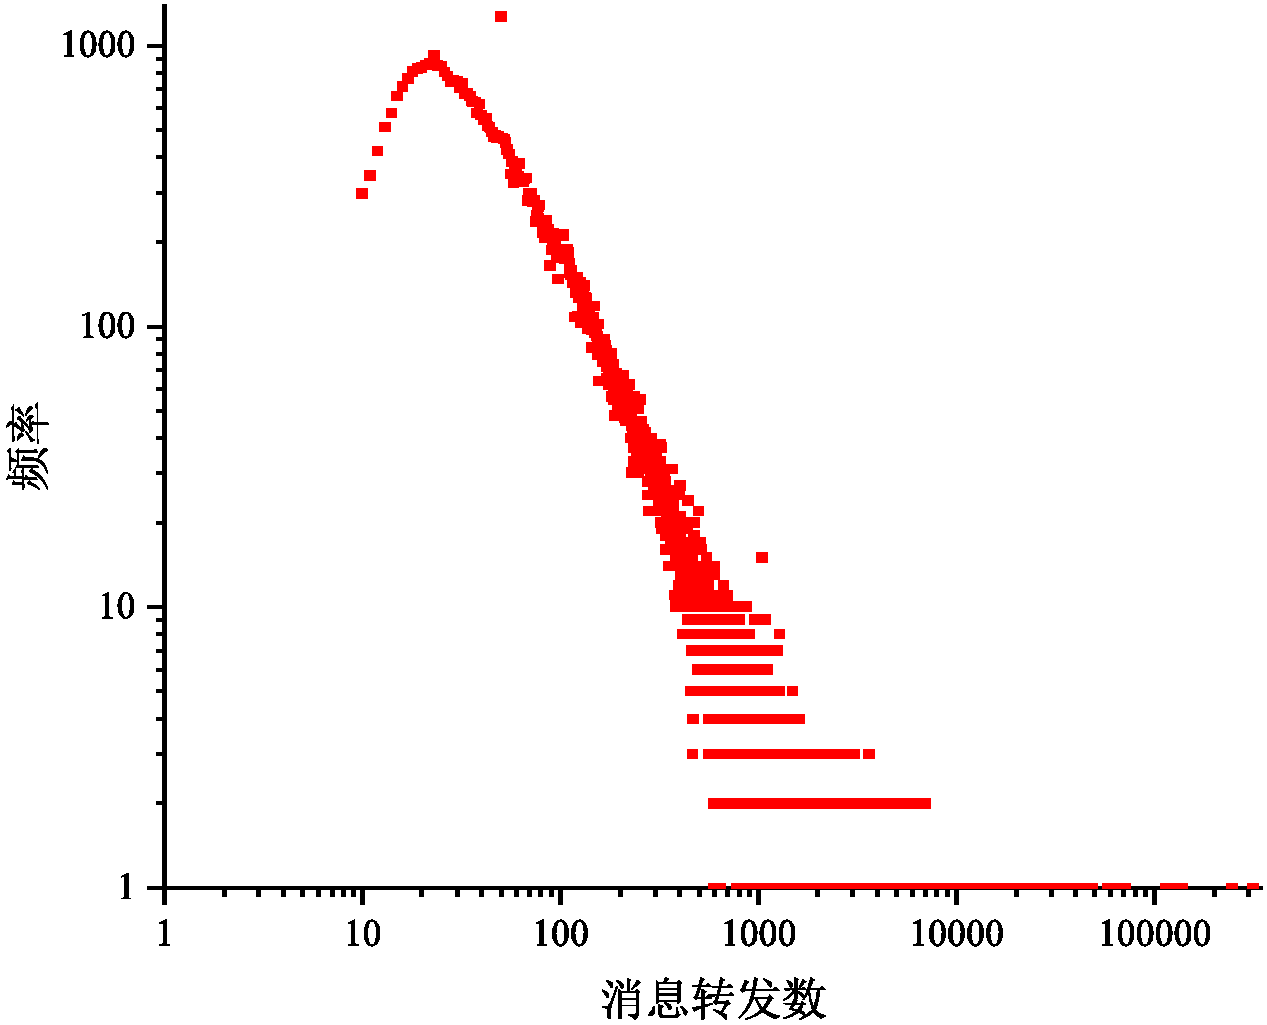
\includegraphics[width=0.8\textwidth]{3-RetweetDist}
  \caption{数据集中消息流行度的分布}
  \label{fig:retweetDist}
\end{figure}

我们将数据集平均分成5 份,轮流选取其中1 份为测试集,剩余4 份为训练集来进行实验。所有展示的实验结果均为5 个测试集的平均结果。
\subsection{实验准备}
\subsubsection{对比模型}
我们选取了以下三个模型来和我们的模型进行对比:
\begin{itemize}
\item 	RPP模型\citep{shen2014modeling}:采用了自增强泊松过程来刻画流行度的到达过程,考虑了消息自己的吸引力、时间衰减效应和富者愈富效应;
\item 	Pinto模型\citep{pinto2013using}:将消息在观测时间窗口内的转发数据表示为时间序列,利用多元线性回归模型来学习时间序列特征与流行度之间的变换函数;
\item SeqSim模型:和我们提出的模型一样,SeqSim 模型也是先从历史消息中寻找到和待预测消息相似的消息,再利用相似消息进行预测。不同于我们的模型,SeqSim模型直接使用时间序列来表示消息的传播数据。
\end{itemize}
\subsubsection{评价指标}
我们使用了平均绝对百分误差(Mean Absolute Percentage Error, MAPE)来度量不同模型的预测效果。模型在预测时间点$t$的MAPE值定义如下:
 \begin{displaymath}
 MAPE(t)=\frac{1}{m}\sum_{i} |\frac{r^i (t)-\widetilde{r^i (t)}}{r^i (t)}|\text{。}
 \end{displaymath}
其中,$m$是测试集的大小,$r^i (t)$表示$t$时刻消息$i$的真实流行度,$\widetilde{r^i (t)}$表示模型对消息$i$在$t$时刻的流行度的预测。MAPE的值越低,表示模型的预测效果越好。
\subsubsection{参数设置}
在我们的实验中,消息的观测窗口设置为1小时,预测窗口设置为24小时。在利用LDA模型学习消息的表示时,LDA的主题数为4时,效果最好,因此实验部分的结果均为主题数为4时的结果。主题数对预测效果的影响将在实验分析章节中进行讨论。在选取最相似的历史消息时,我们将$K$设置为10,即为每条待预测消息找到与之最相似的10条历史消息来进行预测。对于Pinto 模型和SeqSim模型,在生成时间序列时,我们选择的时间区间的长度为5分钟。在使用截尾均值进行预测时,截尾均值的参数$\varepsilon$\%设置为10\%。
\subsection{实验结果}
我们以消息发布后1小时内的转发情况作为观测,来预测后续每隔1小时后消息的流行度情况,实验结果如图\ref{fig:exprResult}所示。
\begin{figure}[!htbp]
  \centering
  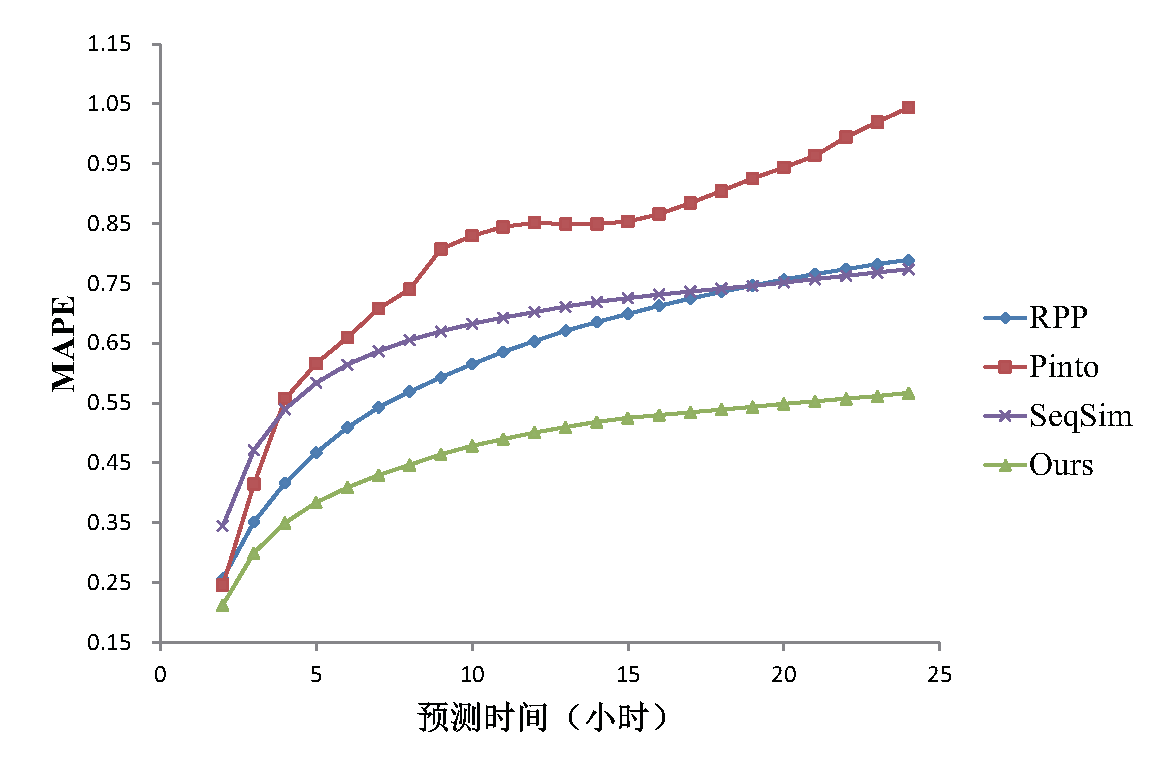
\includegraphics[width=0.8\textwidth]{3-expr}
  \caption{不同模型的流行度预测效果}
  \label{fig:exprResult}
\end{figure}


从图\ref{fig:exprResult}中可以看出,我们提出的模型的预测效果要明显优于其他3个模型。Pinto模型的表现效果最差,因为它用一个模型来预测所有的待预测消息,噪音影响很大。比较Pinto模型和SeqSim模型可以看出,利用相似微博来预测流行度,可以有效地区分出消息本身的特异性,从而显著地提升预测效果。对比SeqSim模型和我们提出的模型的结果可以看出,相比于时间序列的表示方法,我们的提出的基于消息传播模式的表示方法,可以更好地刻画消息的传播过程,进而找到传播过程相似的历史消息来进行预测,得到更精确的预测效果。另外,综合对比两个基于相似消息的模型和其他两个模型,可以发现基于相似消息的模型在进行预测时,随着时间的增长,预测误差的增长更加平稳,预测性能更好。
\subsection{实验分析}
\subsubsection{LDA模型中主题个数的影响}
在利用LDA模型进行表示学习时,主题个数是一个非常重要的超参。我们对不同主题个数设
定下的预测效果进行了实验,结果如图\ref{fig:ldaTopic}所示,其中 表示主题个数, 表示预测时刻。
从图\ref{fig:ldaTopic}可以看出,在不同的预测时间点上,主题个数为4 的模型的预测效果都要明显地由于其他模型,因此,在对比实验中,我们将LDA模型的主题个数设置为4。
\begin{figure}[!htbp]
  \centering
  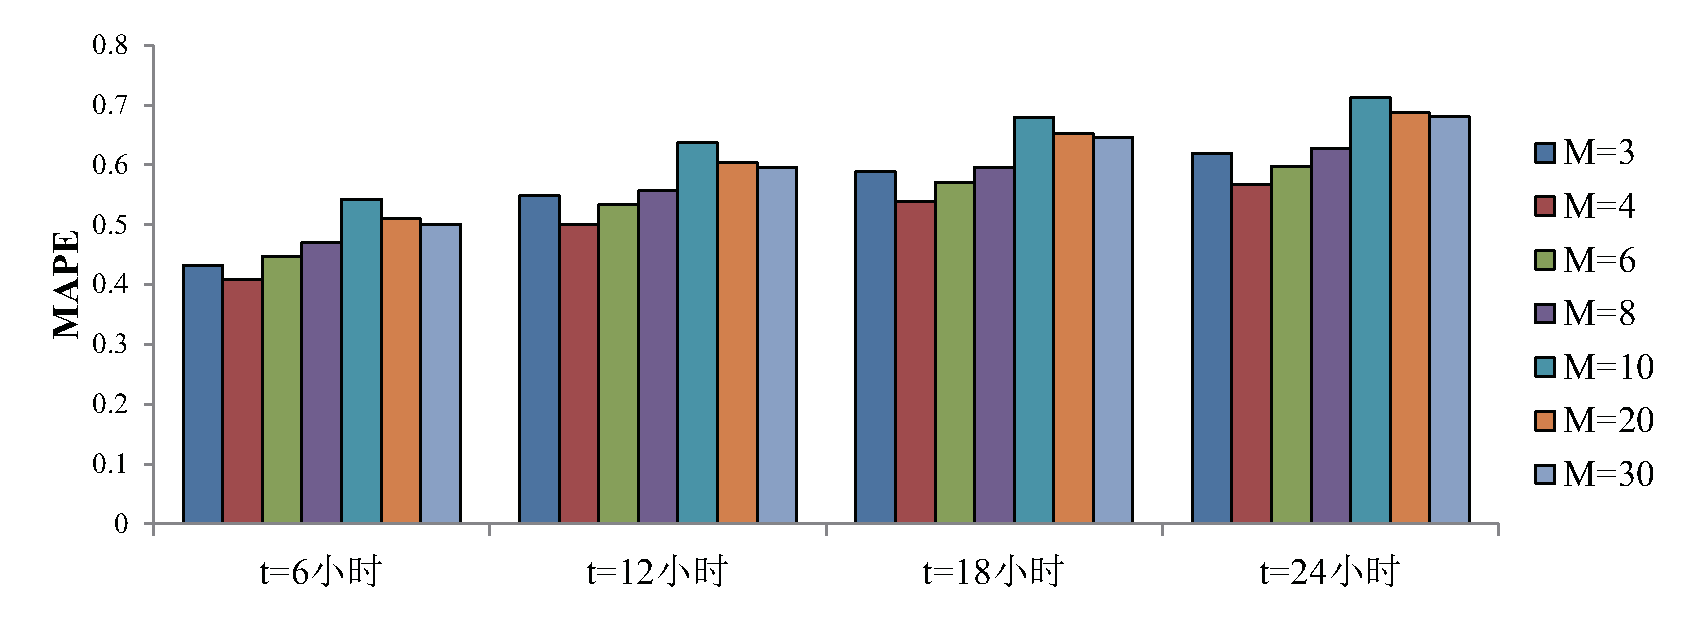
\includegraphics[width=1\textwidth]{3-LDATopic}
  \caption{不同主题数目下模型的预测效果}
  \label{fig:ldaTopic}
\end{figure}

\subsubsection{相似消息分析}
我们在图\ref{fig:simExample}中展示了部分待预测消息以及模型找到与之相似的历史消息的传播数据。图中竖线标识的位置为观测窗口的大小,红点数据标识了待预测消息的流行度变化情况。从图中可以看到,我们找到的相似消息,在观测窗口内的传播过程和流行度大小与待预测消息非常相似;同时在预测时间窗口中,消息的流行度变化趋势也非常一致。这表明我们提出的基于传播模式的表示方法,可以有效地刻画消息的传播过程,从而找到那些变化趋势相近的历史消息来辅助预测。另外,从图中可以看出,找到的近似消息中存在离群点,这也说明了采用截尾平均值的必要性。
\begin{figure}[!htbp]
  \centering
  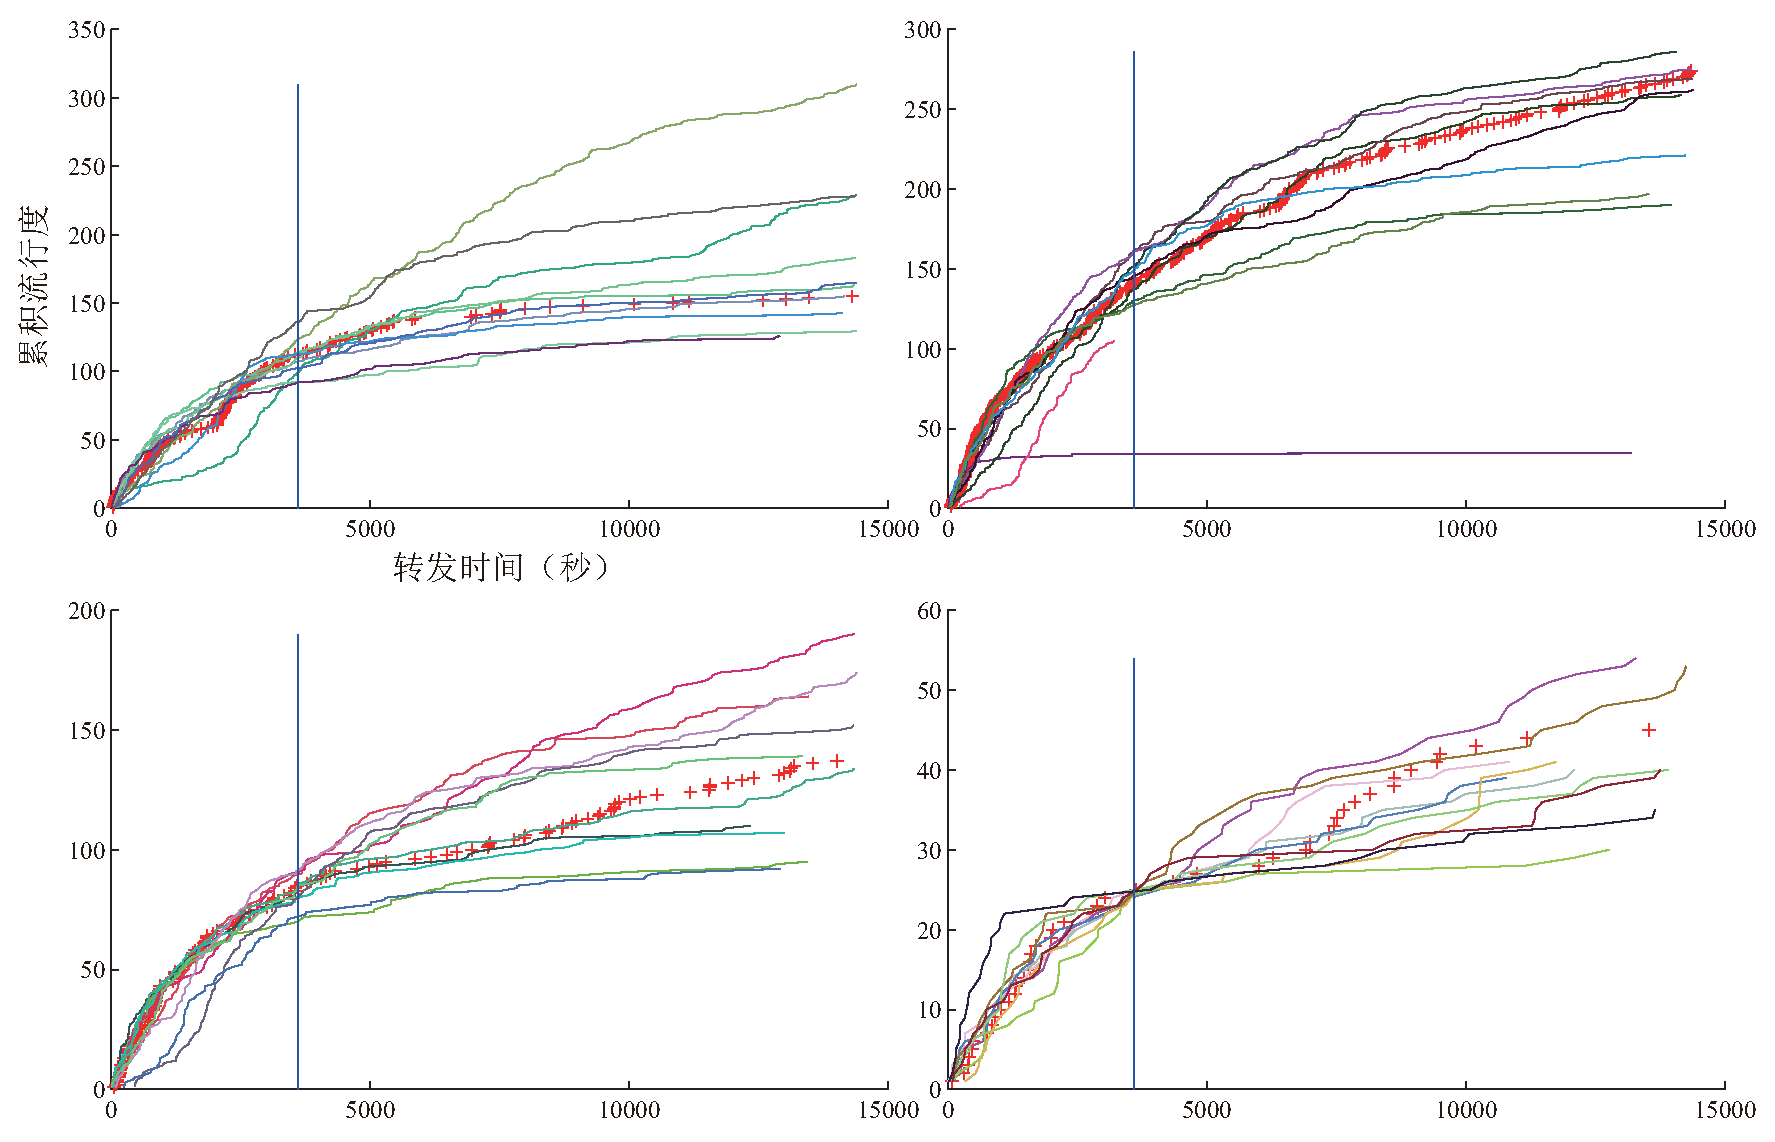
\includegraphics[width=1\textwidth]{3-SimSample}
  \caption{待预测消息及相似微博示例}
  \label{fig:simExample}
\end{figure}

\section{本章小结}
针对现有的两类流行度预测方法的不足,本章中提出了一种基于相似消息的流行度预测方法。对于每一条待预测的消息,我们从历史消息中选取出传播相似度最高的K条消息来进行预测。在计算消息间的相似度时,我们利用了文档主题建模领域的LDA模型,来学习得到消息的表示。我们将消息转发过程中产生的时间间隔数据作为输入,将消息中包含的不同的传播模式作为隐变量,利用LDA模型,学习得到消息在不同传播模式上的分布作为消息的表示。数据集上的实验结果表明,我们的方法能够有效地发现传播模式相近的消息,进而取得了更好的流行度预测效果。

\chapter{面向多中心用户的流行度预测方法}
\label{chap:four}
\section{引言}
\begin{eqnarray}
\label{eq:gradLambda}
\begin{split}
\frac{\partial lnL}{\partial \lambda_l} & = \sum_{i=1}^{n}\frac{f(t_i-t_l)}{\sum_{k=1}^{l} \lambda_k f(t_i-t_k)} + \sum_{i=1}^{n} \int_{0}^{t_i}f(t-t_l)dt - (m+n)\int_{0}^{T}f(t-t_l)dt
\end{split}
\end{eqnarray}

\begin{eqnarray}
\label{eq:gradMu}
\begin{split}
\frac{\partial lnL}{\partial \mu_l} & = \frac{1}{\sigma_l} \cdot \frac{ln(t_i-t_l)-\mu_l}{\sigma_l} \cdot \sum_{i=1}^{n}\frac{\lambda_l f(t_i-t_l)}{\sum_{k=1}^{l} \lambda_k f(t_i-t_k)} \\
& - \frac{1}{\sigma_l} \cdot\lambda_l \sum_{i=1}^{n} \phi(\frac{ln(t_i-t_l)-\mu_l}{\sigma_l}) \\
& + \frac{1}{\sigma_l}\cdot (m+n)\lambda_l \phi(\frac{ln(T-t_l)-\mu_l}{\sigma_l})
\end{split}
\end{eqnarray}

\begin{eqnarray}
\label{eq:gradSigma}
\begin{split}
\frac{\partial lnL}{\partial \sigma_l} & = \frac{1}{\sigma_l} \cdot \sum_{i=1}^{n}\{\frac{\lambda_l f(t_i-t_l)}{\sum_{k=1}^{l} \lambda_k f(t_i-t_k)}[(\frac{ln(t_i-t_l)-\mu_l}{\sigma_l})^2-1]\} \\
& -\frac{1}{\sigma_l} \cdot \lambda_l\sum_{i=1}^{n}\{\phi(\frac{ln(t_i-t_l)-\mu_l}{\sigma_l}) \cdot \frac{ln(t_i-t_l)-\mu_l}{\sigma_l}\} \\
& + \frac{1}{\sigma_l} \cdot (m+n)\lambda_l \phi(\frac{ln(T-t_l)-\mu_l}{\sigma_l}) \cdot \frac{ln(T-t_l)-\mu_l}{\sigma_l}
\end{split}
\end{eqnarray}

\begin{eqnarray}
\label{eq:gradT}
\begin{split}
\frac{\partial lnL}{\partial t_l} &= \frac{1}{t_i-t_l} \cdot \sum_{i=1}^{n}\{ \frac{\lambda_l f(t_i-t_l)}{\sum_{k=1}^l\lambda_kf(t_i-t_k)}(1+\frac{ln(t_i-t_l)-\mu_l}{\sigma_l^2}) \} \\
& -\frac{1}{\sigma_l} \cdot \frac{1}{t_i-t_l}\cdot \lambda_l\sum_{i=1}^{n} \phi(\frac{ln(t_i-t_l)-\mu_l}{\sigma_l}) \\
& +\frac{1}{\sigma_l}\cdot \frac{1}{T-t_l}\cdot (m+n)\lambda_l\phi(\frac{ln(T-t_l)-\mu_l}{\sigma_l})
\end{split}
\end{eqnarray}
\chapter{社交网络中的时间不均匀性建模}
\label{chap:five}
\section{引言}
\section{相关工作}
\chapter{总结与展望}
\label{chap:six}

%%% ++++++++++++++++++++++++++++++++++++++++++++++++++++++++++++++++++++++++++++++++++
%
%%%%% --------------------------------------------------------------------------------
%%
%%%%******************************** Appendix ****************************************
%%
%% Some subordinate chapters.
\cleardoublepage
\appendix%

\chapter{中国科学院大学学位论文撰写要求}
学位论文是研究生科研工作成果的集中体现,是评判学位申请者学术水平、授予其学位的主要依据,是科研领域重要的文献资料。根据《科学技术报告、学位论文和学术论文的编写格式》(GB/T 7713-1987)、《学位论文编写规则》(GB/T 7713.1-2006)和《文后参考文献著录规则》(GB7714—87)等国家有关标准,结合中国科学院大学(以下简称“国科大”)的实际情况,特制订本规定。

\section{学位论文的一般要求}

学位论文必须是一篇(或由一组论文组成的一篇)系统的、完整的学术论文。学位论文应是学位申请者本人在导师的指导下独立完成的研究成果,除论文中已经注明引用的内容外,不得抄袭和剽窃他人成果。对学位论文研究做出重要贡献的个人和集体,均应在文中以明确方式标明。学位论文的学术观点必须明确,且立论正确,推理严谨,数据可靠,层次分明,文字正确、语言通畅,表述清晰,图、表、公式、单位等符合规范要求。

\section{学位论文的水平要求}

硕士学位论文要选择在基础学科或应用学科中有价值的课题,对所研究的课题有新的见解,并能表明作者在本门学科上掌握了坚实的基础理论和系统的专门知识,具有从事科学研究工作或独立担负专门技术工作的能力。

博士学位论文要选择在国际上属于学科前沿的课题或对国家经济建设和社会发展有重要意义的课题,要突出论文在科学和专门技术上的创新性和先进性,并能表明作者在本门学科领域掌握了坚实宽广的基础理论和系统深入的专门知识,具有独立从事科学研究工作的能力。

\section{撰写学位论文的语言及文字}

除外国来华留学生及外语专业研究生外,研究生学位论文一般应采用国家正式公布实施的简化汉字撰写;应采用国家法定的计量单位。学位论文中采用的术语、符号、代号在全文中必须统一,并符合规范化的要求。

外国来华留学生可用中文或英文撰写学位论文,但须采用中文封面,且应有详细的中文摘要。外语专业的学位论文等应用所学专业相应的语言撰写,摘要应使用中文和所学专业相应的语言对照撰写。

为了便于国际合作与交流,学位论文亦可有英文或其它文字的副本。

\section{学位论文的主要组成部分}

学位论文一般由以下几个部分组成:中文封面、英文封面、致谢、中文摘要、英文摘要(Abstract)、目录、正文、参考文献、附录、作者简历及攻读学位期间发表的学术论文与研究成果。

\begin{enumerate}
  \item 学位论文题目应当简明扼要地概括和反映出论文的核心内容,一般不宜超过25个汉字(符),英文题目一般不应超过150个字母,必要时可加副标题。

  \item 论文摘要包括中文摘要和英文摘要(Abstract)两部分。论文摘要应概括地反映出本论文的主要内容,主要说明本论文的研究目的、内容、方法、成果和结论。要突出本论文的创造性成果或新见解,不宜使用公式、图表,不标注引用文献。英文摘要(Abstract)应与中文摘要内容相对应。摘要最后另起一行,注明本文的关键词(3-5个),关键词是为了文献标引工作从论文中选取出来,用以表示全文主题内容信息的单词或术语。

  \item 正文是学位论文的主体,包括引言(或绪论)、论文主体及结论等部分。
    \begin{itemize}
      \item 引言(或绪论)应包括选题的背景和意义,国内外相关研究成果述评,本论文所要解决的问题、所运用的主要理论和方法、基本思路和论文结构等。引言应独立成章,用足够的文字叙述,不与摘要雷同。

      \item 论文主体由于涉及不同的学科,在选题、研究方法、结果表达方式等有很大的差异,不作统一的规定。但必须严格遵循本学科国际通行的学术规范,言之成理,论据可靠,实事求是,合乎逻辑,层次分明,简练可读。

      \item 结论是对整个论文主要成果的总结,应明确、精炼、完整、准确。结论应明确指出本研究的创新点,对论文的学术价值和应用价值等加以预测和评价,说明研究中尚难解决的问题,并提出今后进一步在本研究方向进行研究工作的设想或建议。应严格区分本人研究成果与他人科研成果的界限。
    \end{itemize}

  \item 参考文献应本着严谨求实的科学态度,凡学位论文中有引用或参考、借用他人成果之处,均应按不同学科论文的引用规范,列于文末(通篇正文之后)。需正确区分直接引用和转引并明确加以标注。

  \item 学位论文印刷及装订要求:学位论文用A4标准纸打印、印刷或复印,按顺序装订成册。自中文摘要起双面印刷,之前部分单面印刷。论文必须用线装或热胶装订,不使用钉子装订。学位论文封面采用国科大统一规定的学位论文封面格式,封面用纸一般为150克(需保证论文封面印刷质量,字迹清晰、不脱落),博士学位论文封面颜色为红色,硕士学位论文封面颜色为蓝色。

  \item 学位论文的提交、保存与使用:学位申请者需按规定向国科大提交学位论文的印刷本和电子版,印刷本和电子版在内容与形式上应完全一致;国科大有权保存学位论文的印刷本和电子版,并提供目录检索与阅览服务,可以采用影印、缩印、数字化或其它复制手段保存学位论文;研究所、国科大有义务保护论文作者的知识产权。涉密学位论文在解密后,须按此规定执行。

  \item 本规定自印发之日起施行【2013年04月07日】,解释权属于校学位评定委员会,由国科大学位办公室负责解释。原《中国科学院研究生院研究生学位论文撰写规定》(院发学位字〔2012〕31号)同时废止。
\end{enumerate}
%
%%%%% --------------------------------------------------------------------------------
%%
%%%%******************************* Backmatter ***************************************
%%
%% Matters of Bibliography, Glossary, Index.
\backmatter
%%
%%% >>> Bibliography
%%
\intotoc{\bibname}% add a corresponding item to the contents table and bookmark
\bibliography{Biblio/ref}%
%%
%%% >>> Other contents
%%
%%
%%% >>> Acknowledgements
%%
\chapter{致\quad 谢}

值此论文完成之际,谨在此向多年来给予我关心和帮助的老师、学长、同学、
朋友和家人表示衷心的感谢!

没有~ctex package~的众多前辈的辛勤付出和~CASthesis package~作者吴凌云学长的贡献,
~\LaTeX{}~菜鸟的我是无法完成此学位论文模板的。在~\LaTeX{}~中的一点一滴的成长源于
开源社区的众多资料和教程,在此对所有前辈们的付出表示感谢!

......

谨把本文献给我最敬爱的父亲!

%%
%%% >>> Resume and Published papers
%%
\chapter{作者简历}

\section*{CASthesis~作者基本情况}

吴凌云,男,福建省屏南县人,1975 年出生,中国科学院数学与系统科学研究院博士研究生。

\section*{联系方式}

通讯地址:北京市~2734 信箱,中科院数学与系统科学研究院应用数学所

邮编:100080

E-mail: aloft@ctex.org

\section*{ucasthesis~作者基本情况}

莫晃锐,男,湖南省湘潭县人,1989 年出生,中国科学院力学研究所硕士研究生。

\section*{联系方式}

通讯地址:北京市北四环西路15号中国科学院力学研究所

邮编:100190

E-mail: mohuangrui@gmail.com

\section*{攻读学位期间发表的学术论文及科研成果}

[1] Thesis Template of the University of Chinese Academy of Sciences, 2014.

\section*{项目资助情况}

可以随意添加新的条目或是结构

%%
\end{document}
%%%%% --------------------------------------------------------------------------------
